\documentclass[preprint,12pt]{article}

\usepackage{amsmath,amsthm,amssymb,amsfonts}
\usepackage{graphicx}
\usepackage{textcomp}
\usepackage{multirow}
\usepackage{hyperref}
\usepackage{booktabs}
\usepackage{algorithm}
\usepackage{algpseudocode}
\usepackage{tabularx}
\usepackage{subcaption}
\usepackage[square,numbers]{natbib}
\usepackage{lipsum} % For lipsum
\newtheorem{lemma}{Lemma}



\begin{document}
\pagenumbering{gobble}
%%
%% The "title" command has an optional parameter,
%% allowing the author to define a "short title" to be used in page headers.
\title{A Tiny, Client-Side Classifier}

%%
%% The "author" command and its associated commands are used to define
%% the authors and their affiliations.
%% Of note is the shared affiliation of the first two authors, and the
%% "authornote" and "authornotemark" commands
%% used to denote shared contribution to the research.

\author{C. Meyers, A. P. MacSween, E. Elmroth, and~T. L\"{o}fstedt}

\maketitle


\begin{abstract}
The recent developments in machine learning have highlighted a conflict between online platforms and their users in terms of privacy.
The importance of user privacy and the struggle for power over user data has been intensified as regulators and operators attempt to police the online platforms.
As users have become increasingly aware of privacy issues, client-side data storage, management, and analysis have become a favoured approach to large-scale centralised machine learning.
However, state-of-the-art machine learning methods require vast amounts of labelled user data, making them unsuitable for models that reside client-side and only have access to a single user's data.
State-of-the-art methods are also computationally expensive, which degrades the user experience on compute-limited hardware and also reduces battery life.
A recent alternative approach has proven remarkably successful in classification tasks across a wide variety of data---using a compression-based distance measure (called normalized compression distance) to measure the distance between generic objects in classical distance-based machine learning methods.
In this work, we demonstrate that the normalized compression distance is actually not a metric; develop it for the wider context of kernel methods to allow modelling of complex data; and present techniques to improve the training time of models that use this distance measure.
We show that the normalised compression distance works as well as and sometimes better than other metrics and kernels---without incurring additional computational costs and in spite of the lack of formal metric properties.
The end results is a simple model with remarkable accuracy even when trained on a very small number of samples allowing for models that are small and effective enough to run entirely on a client device using only user-supplied data.
\end{abstract}





\section{Introduction}

Modern machine learning (ML) methods have demonstrated remarkable efficacy across many domains.
However, they often have large numbers of parameters, and thus also require large numbers of samples to train on~\cite{desislavov2021compute}.
This aggregation of vast amounts of data creates numerous privacy, safety, and security threats~\cite{chat_control} that are consequences of large-scale user data collection, for instance by online platform operators (see Section~\ref{threat} for more details).
We evaluate and extend prior work on compression-based distance measures by incorporating them into novel kernel methods, enabling efficient classification even with limited training samples.
When using small training sets and small and efficient models, they can be trained entirely on a client device without sharing private user data with anyone---allowing the model builder to circumvent many weaknesses associated with state-of-the-art methods~\cite{chat_control,power_consumption_ai,desislavov2021compute}.
We demonstrate the efficacy of the proposed approach in the context of malware detection, network intrusion detection, and spam detection.

\subsection{Threat Model}
\label{threat}

In the context of online platforms, data are collected from end-users using dubious amounts of consent~\cite{nouwens2020dark} and aggregated at massive scales~\cite{desislavov2021compute}.
Such data collection on online platforms often creates privacy, safety, and security risks~\cite{chakraborty_adversarial_2018,meyers}.
One such privacy risk is the periodic attempts by regulators to weaken encryption standards~\cite{amnesty_encryption} and create backdoors to user devices.
Platform operators and governments discuss best-practices for scanning client devices for illegal or ``offensive''
content~\cite{chat_control,apple_csam}, but existing proposals are no less risky to user privacy, safety, or security than weakening encryption.
Privacy experts have denounced such approaches for numerous reasons: the ease of \textit{extracting} private training data~\cite{choquette2021label,fredrikson_model_2015,li2021membership} or the model itself~\cite{fredrikson_model_2015,orekondy2019knockoff,jagielski2020high,correia2018copycat,shokri2017membership}, the ability of a malicious user to induce false positives for other users when the model is trained on user data~\cite[\textit{poisoning} attacks;][]{rawat2022devil,shokri2020bypassing,gu2017badnets,saha2020hidden,aghakhani2021bullseye,turner2018clean,shafahi2018poison,geiping2020witches,souri2022sleeper}, and the triviality of simply \textit{evading} the detection mechanism~\cite{carlini_towards_2017,dohmatob_generalized_2019,hopskipjump,biggio_evasion_2013,meyers,chakraborty_adversarial_2018,deepfool,hopskipjump}.

Current platform solutions often rely on large-scale ML methods that are trained on vast amounts of user data and federated across devices~\cite{apple_csam}---an approach that has been criticized by privacy experts~\cite{chat_control}.
Examples of security risks include attacks against ML systems that target a model during training~\cite{biggio_poisoning_2013}, prediction~\cite{biggio_evasion_2013,deepfool,carlini_towards_2017}, and deployment~\cite{distributed_attacks,santos2021universal}.
Even when access to a model by an adversary is limited, it is possible to induce a misclassification~\cite{hopskipjump}, reverse engineer the model~\cite{extraction_attack}, determine the model weights~\cite{jagielski2020high}, or infer the class-membership of new samples~\cite{bentley2020quantifying}.
This raises profound questions for safety-critical systems~\cite{meyers} and legal questions about access and control of the underlying data~\cite{mitrou2018data,marks2023ai}.
Additionally, it has been shown that finding prototypical meta samples from the training set of large-scale ML models is trivial~\cite{trashfire,meyers}.
Even if the attacker only has access to a typical application programming interface (API), there are reliable ways to fool the model~\cite{hopskipjump}.

Many privacy experts warn of the potential for any hypothetical \textit{centralized} content-censoring system not only because of the potential failures due to adversaries mentioned above, but also because of the potential these systems to be used for mass surveillance and censorship~\cite{chat_control}.
In short, distributed and centralised training paradigms are both inherently fragile to malicious users and dangerous for user privacy, even if the resulting model lives on the user device (rather than in the cloud).


\subsection{Motivations}

In contrast to many state-of-the-art methods, this work proposes a light-weight, client-side approach to content filtering that does not rely on large-scale data collection.

Recently, Jiang \textit{et al.}~\cite{jiang2022less} proposed a remarkably successful approach to ``parameter free'' classification, dubbed NCD-KNN, that exploits a compress\-ion-based distance measure, the \textit{normalized compression distance}~\citep[NCD;][]{ncd}, to classify objects using the $k$-nearest neighbours (KNN) method~\cite{shalev2014understanding}.
NCD-KNN is known to work well even when trained on small numbers of samples~\cite{scilipoti2024strong}.
By building a model that is accurate on a small number of samples, we can fulfil the goal of training a ML model entirely on a client device using data generated by a single user.
An additional goal of this work was to evaluate the efficacy of NCD in general and to extend it to kernel methods in particular.

While other research examined topics like image classification~\cite{opitz2023gzip}, molecular property classification~\cite{weinreich2023parameter}, and text classification~\cite{nishida2011tweet}, the ability of NCD to classify datasets that contain strings, numeric values, and categorical data (heterogenous datasets) has remained unexplored.

Additionally, the original NCD work~\cite{ncd} included an error term that is usually ignored in recent research~\cite{opitz2023gzip,weinreich2023parameter,nishida2011tweet,jiang2022less}.
To the best of our knowledge, no research has addressed the problem of negative values for NCD\@.
The original authors~\cite{ncd} asserted that NCD is always positive when using perfect compressors.
However, this is clearly demonstrated to be false in Lemma~\ref{pseudometric} when using imperfect compressors (which is what we will have in practice).

Prior works about NCD have primarily focused on distance-based ML methods (\textit{e.g.}, KNN), which limits both the class of methods that can be considered and the types of data that can be effectively analysed.
A key motivation for this work was to extend the use of NCD beyond distance-based methods by developing a novel kernel-based formulation. This significantly broadens the applicability of NCD, making it suitable for a wider range of machine learning techniques where traditional distance-based approaches cannot be used.



\subsection{Contributions}

To use NCD, the model builder must choose a compression algorithm.
While the effect of various compressors has been explored, in part, before~\cite{ncd_pitfalls}, we expand the analysis by Cebri\'{a}n \textit{et al.}~\cite{ncd_pitfalls} to more recent compression algorithms and also offer additional run-time improvements over previous implementations~\cite{jiang2022less}.

The NCD-KNN method has shown very strong performance across several benchmarks, but prior implementations~\cite{jiang2022less} are not appropriate for real-time settings due to unnecessary repeated computations.
We therefore propose several run-time improvements and modifications, outlined in Section~\ref{improvements}.

Further, we show that NCD is not a metric~\cite{opitz2023gzip,weinreich2023parameter,nishida2011tweet,jiang2022less}, which means that applying ML methods blindly can lead to erroneous results (\textit{e.g.}, by incorrectly ordering the nearest neighbours).
In this work we demonstrate this non-metric behaviour in Lemma~\ref{pseudometric} and propose techniques to mitigate the effects of this behaviour in Section~\ref{improvements}, effectively making the modified NCD ``more like a metric''.

Additionally, we expand the notion of NCD~\cite{opitz2023gzip,weinreich2023parameter,nishida2011tweet,ncd,jiang2022less,jiang2022less} to kernels (Section~\ref{kernels}) thus allowing for this method to be used with other models besides KNN\@.
We thus extend NCD to reproducing kernel Hilbert spaces and hence more elaborate ML methods---allowing its use in a broader set of ML methods and to model more complex decision boundaries.

Hence, in this paper, we:

\begin{itemize}
    \item Demonstrate that the normalized compression distance is not a metric (Lemma~\ref{pseudometric}) and propose techniques to make it behave ``more like a metric'' (Section~\ref{symmetrisation}).
    \item Propose the use of NCD as a kernel and evaluate its efficacy.
    % \item Discuss how private model deployment is safer by design (Section~\ref{threat}) and the efficacy of this design-constraint on several datasets (see Figure~\ref{fig:sample_size}).
    \item Develop classifiers (evaluations with KNN, logistic regression, and support vector machines (SVC)) that offers large run-time improvements over a reference implementation~\cite{jiang2022less} (Section~\ref{improvements}).
    % \item Provide efficient implementations of the proposed classifiers in \texttt{Java\-script} as well as a \texttt{Scikit-learn} compatible implementation in \texttt{Python}.
    \item Evaluate and empirically show the efficacy of the proposed NCD-based classifiers across multiple binary classification tasks (Section~\ref{results}).
\end{itemize}



\section{Background}

In the sections below, we describe and define the NCD, outline the NCD-KNN method proposed by Jiang \textit{et al.}~\cite{jiang2022less}, outline several other string metrics, and discuss the distance matrix and how to efficiently compute it,



\subsection{Normalized Compression Distance}
\label{ncd}

NCD has been demonstrated to be a \textit{universal} measure of similarity between two objects~\cite{ncd}---where a value of 0 denotes equivalence and a value of 1 denotes complete dissimilarity.
The NCD is defined as~\cite{ncd}
\begin{equation}
    \text{NCD}(x, x') = \frac{|\mathcal{C}(xx')| - \min\{|\mathcal{C}(x)|, |\mathcal{C}(x')|\}}{\max\{|\mathcal{C}(x)|, |\mathcal{C}(x')|\}} + \varepsilon,
    \label{eq:ncd}
\end{equation}
where $|\mathcal{C}(z)|$ is the length of the compressed form of the data, $z$, using compression algorithm, $\mathcal{C}$, the notation $xx'$ denotes the concatenation of strings $x$ and $x'$, and $\varepsilon\geq0$ is an error term accounting for imperfect compression algorithms~\cite{ncd}. The error term is usually assumed to be small relative to the other term.

NCD requires a choice of compression algorithm, and we evaluated the \texttt{gzip}~\cite{gzip}, \texttt{bz2}~\cite{bz2}, and \texttt{brotli}~\cite{google} compressors.
To distinguish between the use of these different compressors, a subscript is used such that NCD$_{\text{gzip}}$ denotes the use of the \texttt{gzip} compressor.
% section{NCD is a not a metric}

While NCD is often discussed as a measure of distance~\cite{opitz2023gzip,weinreich2023parameter,nishida2011tweet,jiang2022less,ncd}, it does in fact not adhere to the axioms of metric spaces.
A function, $d:X \times X \rightarrow \mathbb{R}$, associated with a set of points, $X$, where $\mathbb{R}$ denotes the set of real numbers, is said to be a metric if the following four axioms hold for all $x_1, x_2, x_3 \in X$~\cite{metrics}:
\begin{align}
    \text{Zero Axiom:} \quad & d(x_1,x_2) = 0 \iff x_1 = x_2 \label{eq:axiom_zero} \\
    \text{Non-negativity Axiom:} \quad & d(x_1,x_2) \geq 0 \label{eq:axiom_nonnegativity} \\
    \text{Symmetry Axiom:} \quad & d(x_1,x_2) = d(x_2, x_1) \label{eq:axiom_symmetry} \\
    \text{Triangle Inequality:} \quad & d(x_1,x_3) \leq d(x_1,x_2) + d(x_2,x_3) \label{eq:axiom_triangle}.
\end{align}

Much of the literature devoted to NCD has treated it as a proper metric~\cite{opitz2023gzip,weinreich2023parameter,nishida2011tweet,jiang2022less}.
However, as we show now, it is not.

\begin{lemma}
    When using \texttt{gzip}, \texttt{bz2}, and \texttt{brotli} compressors, NCD does not adhere to the axioms in Equations~\ref{eq:axiom_zero}--\ref{eq:axiom_triangle}, and is thus not a metric.
    \label{pseudometric}
\end{lemma}
\begin{proof}


    We show in what follows that NCD fails to adhere to the axioms for metrics by counter-examples.

    \vspace{0.5em}
    \noindent%
    \textit{Zero axiom:} The following counter-examples violate the zero axiom:
    $$
    \text{NCD}_{\text{gzip}}(A,A) = 0.05,~~\text{NCD}_{\text{bz2}}(B,G) = 0,~~\text{and~~NCD}_{\text{brotli}}(X,X) = 0.2.
    $$

    \vspace{0.5em}
    \noindent%
    \textit{Non-negativity axiom:} The following counter-examples violate the non-nega\-tivity axiom:
    $$
        \text{NCD}_{\text{gzip}}(AAAA,AAAA) = -0.04,
    $$
    $$
        \text{NCD}_{\text{bz2}}(AABABAA,BAABAAB) = -0.03,
    $$
    and
    $$
        \text{NCD}_{\text{brotli}}(CCCCBBCCC, CBCCCBBCCC) = -0.08.
    $$

    \vspace{0.5em}
    \noindent%
    \textit{Symmetry axiom:} The following counter-examples violate the symmetry axiom:
    $$
        \text{NCD}_{\text{gzip}}(AA, BAA) = 0.13 \neq \text{NCD}_{\text{gzip}}(BAA, AA) = 0.04,
    $$
    $$
        \text{NCD}_{\text{bz2}}(AA, AAB) = 0.11 \neq \text{NCD}_{\text{bz2}}(AAB, AA) = 0.00,
    $$
    and
    $$
        \text{NCD}_{\text{brotli}}(AAAAAAA, B) = 0.6 \neq \text{NCD}_{\text{brotli}}(B, AAAAAAA) = 0.7.
    $$

    \vspace{0.5em}
    \noindent%
    \textit{Triangle Inequality:} The following counter-examples violate the triangle inequality:
    $$
        \text{NCD}_{\text{gzip}}(AAA, A) > \text{NCD}_{\text{gzip}}(AAA, AAAA) + \text{NCD}_{\text{gzip}}(AAAA, A),
    $$
    $$
        \text{NCD}_{\text{bz2}}(BC, AN) > \text{NCD}_{\text{bz2}}(BC, J) + \text{NCD}_{\text{bz2}}(J, AN),
    $$
    and if
    $$
     x_1 = CAAAACAA,~~x_2 = CAC,~~\text{and}~~x_3 = CCACCCACCC,
    $$
    then
    $$
        \text{NCD}_{\text{bz2}}(x_1,x_3) > \text{NCD}_{\text{bz2}}(x_1,x_2) + \text{NCD}_{\text{bz2}}(x_2,x_3).
    $$
\end{proof}



\subsection{Other String Metrics}
\label{other_string_metrics}
To model datasets that comprise strings, several existing measures of distance between strings are routinely used~\cite{levenshtein}.
To evaluate the relative performance of the NCD metric, we compared it to several other common measures of string distance:
% String Distances
\begin{itemize}
    \item \textit{Levenshtein} is the ``edit distance'' or minimum number of single-character edits to transform one string into another~\cite{navarro2001guided}.
    \item \textit{Lev Ratio} is the Levenshtein distance divided by the total length of the longer string~\cite{levenshtein}.
    \item \textit{Hamming} is the number of character positions where two strings differ.
    \item \textit{Ham Ratio} is the number of character positions where two strings differ, divided by the length of the longer string.
\end{itemize}


\subsection{Calculating the distance matrix}
\label{distance_matrix}

In what follows, the pairwise distances between two sets of samples (denoted $X$ and $X'$) is collected in a a \textit{distance matrix}, $D$.
When computing the value of NCD$(x,x')$, it is necessary to calculate the values of $\mathcal{C}(x)$ and $\mathcal{C}(x')$.
To classify a sample, Jiang \textit{et al.}~\cite{jiang2022less} iterated over all elements in the sets $X$ and $X'$, where $X$ would be a set of samples with known labels and $X'$ one with unknown labels, such that for each $x_i \in X$ the compression $\mathcal{C}(x_i)$ was computed repeatedly for each $x_j' \in X'$.
Because computational time scales linearly with the size of both $X$ and $X'$, the run time is thus $\mathcal{O}(|X|\cdot|X'|)$ for both compute and memory, where $|X|$ is the cardinality of the set $X$.
Clearly, if the number of samples in $X$ and $X'$ are large, then run-time becomes a concern.
We propose some modifications to how the pairwise distances are computed and which pairwise distances are computed to reduce the computational costs and also make NCD behave ``more like a metric'', which is outlined in Section~\ref{improvements}.





\section{Methods}
\label{methods}

This section outlines proposed modifications to NCD and Jiang's NCD-KNN method~\cite{jiang2022less} before outlining the data and experiments used to verify the efficacy of said modifications.



\subsection{Proposed Modifications to NCD}
\label{improvements}

Jiang \textit{et al.}'s implementation of the NCD-KNN method~\cite{jiang2022less} becomes inefficient because it includes many repeated computations.
To minimize run-time, we first propose a simple improvement in Section~\ref{pre_compute_compression}.
Second, we propose several modifications that symmetrise the distance matrix, intended to ensure adherence to the symmetry axiom (Equation~\ref{eq:axiom_symmetry}).
Then, in an effort to improve the adherence to the zero axiom (Equation~\ref{eq:axiom_zero}) we propose a modification for the special case of $x=x'$ in Section~\ref{zero_check}.
Finally, we outline the proposed way to use NCD as a kernel in Section~\ref{kernels}.


\subsubsection{Pre-computing the Compression vector}
\label{pre_compute_compression}

When computing the value of NCD$(x,x')$, it is necessary to calculate the values of $\mathcal{C}(x)$ and $\mathcal{C}(x')$ as in Equation~\ref{eq:ncd}.
For each $x \in X$, the $\mathcal{C}(x)$ would be computed repeatedly when computing the pairwise NCD distances between $x\in X$ and the elements in $X'$.
Instead of recomputing the $\mathcal{C}(x)$ repeatedly, it is much more efficient to pre-compute the compressed versions of each element in $X$ and $X'$ only once.
Since compressing the input samples is the most costly part of this computation, this saves substantial run-time as demonstrated in Section~\ref{results}.


\subsubsection{Symmetrisation}
\label{symmetrisation}

We propose three new ways to induce ``more'' adherence to the axioms in Equations~\ref{eq:axiom_zero}--\ref{eq:axiom_triangle} and compare their efficacy and run-time in Section~\ref{results}.

For the purposes of the experiments below, the method proposed by Jiang \textit{et al.}~\cite{jiang2022less} is denoted ``Vanilla'' and computes the pairwise distances between two sets by naively computing every element of a distance matrix using the NCD function in Equation~\ref{eq:ncd}.

The second method, proposed here as a modification to NCD, assumes symmetry by only computing the lower triangular part of the distance matrix and then reflecting those values about the diagonal, instead of computing the entire distance matrix; this method is denoted ``Assumed.''
Hence, in a distance matrix, $D$, the ``Assumed'' method computes the lower triangular part of $D$ and then let
\begin{equation}
    D_{i,j} = D_{j,i},
    \label{eq:assumed}
\end{equation}
which effectively halves the computational cost of computing the distance matrix.

In the third method, proposed here, symmetry is \textit{enforced} by sorting the inputs of NCD alphanumerically before computing the distance between them.
This approach thus ensures symmetry during prediction as well as training.
This method is denoted ``Enforced'', and also effectively halves the computational cost of computing the distance matrix since again $D_{i,j} = D_{j,i}$.

The fourth method, also proposed here, computes the \textit{average} value of $\text{NCD}(x,x')$ and $\text{NCD}(x',x)$.
The average of $\text{NCD}(x,x')$ and $\text{NCD}(x',x)$ is
\begin{equation}
    \label{eq:naive_average_symmetrisation}
    \overline{\text{NCD}}(x,x') = \frac{\text{NCD}(x,x') + \text{NCD}(x', x)}{2},
\end{equation}
which can be simplified to
\begin{equation}
    \label{eq:simplified_average_symmetrisation}
    \overline{\text{NCD}}(x, y) = \frac{\frac{\mathcal{C}(xx') + \mathcal{C}(x'x)}{2} - \min[\mathcal{C}(x), \mathcal{C}(x')]}{\max[\mathcal{C}(x), \mathcal{C}(x')]} + \varepsilon,
\end{equation}
which clearly leads to $D_{i,j}=D_{j,i}$.
The simplification in Equation~\ref{eq:simplified_average_symmetrisation} thus only includes one additional compression, increasing the computational cost by roughly 20\% instead of doubling the computational cost as in Equation~\ref{eq:naive_average_symmetrisation}. This method is denoted ``Averaged''.


\subsubsection{Zero-axiom check}
\label{zero_check}

A simple means to ensure that the output of NCD is zero when the two inputs are equal, we propose to check for this case before any distances are computed and return zero if the inputs are equal.
We denote this modification the ``Zero-axiom check''.
The Zero-axiom check was performed with the ``Assumed'' and ``Enforced'' methods, but not the ``Averaged'' method, assuming that the error associated with calculating NCD$(x,x')$ would cancel out the error associated with NCD$(x,x')$.



\subsection{Kernelisation}
\label{kernels}

We propose to use NCD to construct an approximate kernel, allowing NCD to be used with a much larger set of ML methods than as a distance.
For this purpose, a kernel is defined as a function, $k : X \times X \rightarrow \mathbb{R}$, such that
\begin{equation}
    k(x, x') := \langle \phi(x), \phi(x') \rangle
    \label{eq:kernel}
\end{equation}
for all $x, x' \in X$,
where $\phi: X \to Y$ is a feature function (a function extracting features from its inputs), and $\langle \cdot, \cdot \rangle$ denotes an inner product in the feature space, $Y$.
The $i$-th row and $j$-th column of a kernel matrix, $K$, is
$$
    K_{ij} = k(x_i, x_j).
$$

The radial basis function (RBF) kernel~\cite{shalev2014understanding}, also known as the Gaussian kernel (when the distance is the Euclidean distance) is defined as
\begin{equation}
    k(x, x') = \exp\left(-\frac{d{(x, x')}^2}{\lambda}\right),
    \label{eq:rbf_kernel}
\end{equation}
where $\lambda$ is a tunable parameter (denoted a \textit{length scale}) that controls how quickly the kernel function decreases as a function of the distance between points, \textit{i.e.}, determines the influence of individual points on neighbouring points.
We thus propose to use NCD as the distance function, $d$, in the kernel in Equation~\ref{eq:rbf_kernel}.
The RBF kernel is particularly effective as it is known to be a universal function approximator~\cite{rbf_universal}.

The Hamming kernel~\cite{hamming_kernel}, based on the Hamming distance between two strings or binary vectors, is defined as
\begin{equation}
    k(x, x') = 1 - \lambda \frac{d_H(x,x')}{\max(|x|,|x'|)},
    \label{eq:hamming_kernel}
\end{equation}
where $ d_H(x, x') $ denotes the Hamming distance, $\max(|x|,|x'|)$ denotes the length of the longer string, and $ \lambda $ is a tunable parameter that controls the sensitivity of the kernel to differences between input vectors.
Smaller values of $ \lambda $ cause the kernel to decay more rapidly as the number of differing positions increases, thereby emphasizing exact or near-exact matches.
We propose to use this kernel in settings where inputs are strings or binary representations, as it naturally captures similarity through positional agreement.
Like the RBF kernel, the Hamming kernel belongs to the class of positive-definite kernels and has been shown to be effective at classification tasks~\cite{hamming_classification}.

% To use such a kernel with the outlined string distances, however, a pairwise distance matrix between all samples must be precomputed.

Euclidean distances can be computed in the feature space by using a kernel. We see that
\begin{align*}
    d(x,x')
        &= \| \phi(x) - \phi(x') \|_2^2 \\
        &= \langle\phi(x) - \phi(x'), \phi(x) - \phi(x') \rangle \\
        &= \langle \phi(x), \phi(x) \rangle + \langle \phi(x'), \phi(x') \rangle - 2\langle \phi(x), \phi(x') \rangle \\
        &= k(x, x) + k(x', x') - 2k(x, x'),
\end{align*}
and denote this distance as the \textit{kernel distance}.
For the RBF kernel, when the symmetry and the zero axioms hold, we have that $k(x,x) = k(x',x') = 1$, and the kernel distance can be computed efficiently as
\begin{equation}
    d_k(x, x') = 2 - 2 k(x, x').
    \label{eq:kernel_distance}
\end{equation}
This formulation was used to extend NCD-KNN to kernels, \textit{i.e.}, the kernel distance in Equation~\ref{eq:kernel_distance} was used together with the RBF kernel in Equation~\ref{eq:rbf_kernel}, as well as with the Hamming kernel in Equation~\ref{eq:hamming_kernel}.
Logistic regression and SVCs were trained on the kernel matrices formed from Equations~\ref{eq:rbf_kernel}~\&~\ref{eq:hamming_kernel}.


\subsection{Data}
\label{datasets}

Several open datasets were used to evaluate the efficacy of NCD in the context of heterogeneous tabular and text data.

We used the KDD-NSL data, which is a log of system process data for both regular users (denoted benign) and malicious software (denoted adversarial)~\cite{kddnsl}. It includes 6072 samples and 41 features that encapsulate the behaviour of both benign software and malware.
KDD-NSL includes software protocol, system error rate, whether the process has root privileges, and the number of files accessed by the process.

We also used the DDoS IoT dataset~\cite{ddos}, which includes information collected from network packet headers of adversarial and benign users across many types of DDoS attacks.
Specific features include source IP address, source port, destination IP address, destination port, and network protocol among a total of 90 features across more than 40 million samples, collected from both benign users and malicious traffic.
% To prepare the DDoS IoT dataset, the timestamp data was removed since the malicious and benign data were collected at different times and necessarily encodes the class label.

We used the Truthseeker dataset~\cite{truthseeker}, which includes 134 thousand messages from Twitter users with a label provided by the data distributors, and a label that encodes whether or not a given user was a suspected bot.
% While this dataset is normally includes metadata-- in an effort to examine the efficacy of NCD on text alone-- this work only included the ``tweet" and the ``BotScoreBinary'' label provided by the researchers who distribute the data (the classes represent regular users and suspected bot users).

Finally, we used the SMS Spam dataset~\cite{sms_spam} which includes SMS messages and a label indicating whether or not a message is spam across 5575 samples.

For several of the datasets, malicious examples were rare compared to the number of benign examples. To address the class imbalances, each dataset was under-sampled~\cite{undersampling} using the \texttt{imblearn} package~\cite{imblearn} to reduce bias towards the majority class and to ensure metrics like accuracy are meaningful.
For each dataset, model, symmetrisation method, and distance metric, 1000 samples from each dataset were used to conduct five-fold cross validation, yielding five disjoint validation sets of 200 samples each.
Accuracy, distance matrix computation time, model training times, and prediction times were recorded for each of the five cross-validation folds.
In an effort to represent both text and numerical data as strings, the rows of each numerical dataset were extracted as lists in \texttt{Python} and then those lists were cast directly to strings for the DDoS, KDD-NSL, and SMS Spam datasets.

\subsection{Experiments}
\label{experiments}

We evaluated the proposed methodology using the described datasets, models, symmetrisation methods (``Vanilla'', ``Assumed'', ``Enforced'', and ``Averaged''), and metrics ($\text{NCD}_{\text{gzip}}$, $\text{NCD}_{\text{bz2}}$, and $\text{NCD}_{\text{brotli}}$, Levenshtein distance, a normalised Levenshtein distance (labelled Lev Ratio),  Hamming distance, and a normalised Hamming distance (labelled Ham Ratio)).
After generating the 5-fold cross validation sets for each dataset, the distance matrices for each symmetrisation method and metric were computed, as outlined in Sections~\ref{distance_matrix} and~\ref{symmetrisation}.
Additionally, kernel matrices were computed as described in Section~\ref{kernels}.
The classifiers used were KNN, logistic regression, and SVC, as implemented in \texttt{scikit-learn}~\cite{sklearn}.
For KNN, we both used NCD directly and used the kernel distance from Equation~\ref{eq:kernel_distance} computed using both the RBF and Hamming kernels.
For (kernel) logistic regression and SVC, the RBF kernel in Equation~\ref{eq:rbf_kernel} and the Hamming kernel in Equation~\ref{eq:hamming_kernel} were used with the NCD distance.

Each model was tuned using the hyper-parameters outlined in the following.
For NCD, all metrics (NCD, Hamming distance, Levenshtein distance, etc) were used to compute kernel matrices as per Equations~\ref{eq:rbf_kernel}~and~\ref{eq:kernel_distance}.
In addition, the Hamming kernel from Equation~\ref{eq:hamming_kernel} was used as a baseline~\cite{hamming_kernel}.
Both kernels have a hyper-parameter, $\lambda$, that must be tuned; $\lambda$ was was evaluated in powers of 10 in the range $[10^{-3}, 10^3]$.

KNN requires the model builder to specify the number of nearest neighbours.
In our experiments, $k \in \{1,3,5,7,11\}$, as odd numbers means there were no ties (for our binary classification task).
In logistic regression, an $\ell_2$ penalty was used as well as a configuration without any penalty.
The coefficient of the penalty was set to powers of 10 in the range $[10^{-3}, 10^3]$.
The \texttt{SAGA} solver~\cite{saga} was used for logistic regression, with a tolerance of $10^{-4}$.
The penalty term in the SVC was varied in the range $[10^{-3}, 10^3]$ for each power of ten.

To find the most appropriate set of hyper-parameters, each of the dataset-model-symmetrisation-metric combinations enumerated above were evaluated using a grid search and 5-fold cross-validation.
Then, the best-fit model was chosen for each dataset-model-symmetrisation-metric configuration by finding the configuration(s) with the highest mean cross-validation accuracy and choosing the model with the smallest standard deviation in the case ties.
After fitting each model to each dataset, symmetrisation method, measure of distance, and model-dependent hyper-parameters, the best-fit models were repeatedly trained on $m \in \{10, 20, 35, 60, 100, 200, 500, 1000\}$ samples and evaluated against the 200 withheld samples during cross-validation to evaluate the ability of the model to generalise even when trained on a small number of samples.

In addition to the classification experiments above, the distance matrices calculated from those datasets were exhaustively checked for adherence to the axioms in Equations~\ref{eq:axiom_zero}--\ref{eq:axiom_symmetry} and the percentage of violations for each axiom was recorded.
In addition, 100k randomly selected 3-tuples from each distance matrix were sampled to compute the percentage of samples that violate Equation~\ref{eq:axiom_triangle}.
An additional synthetic dataset comprised of 100k 3-tuples was generated from short, alphabetic strings using the uppercase English alphabet and a maximum string size of 144 characters (the length of a ``tweet'') for each metric and symmetrisation method and used to calculate the probability of axiom violations.


\section{Results and Discussion}
\label{results}

In this section, the results from the aforementioned experiments are discussed.

\begin{figure}[!htb]
    \centering
    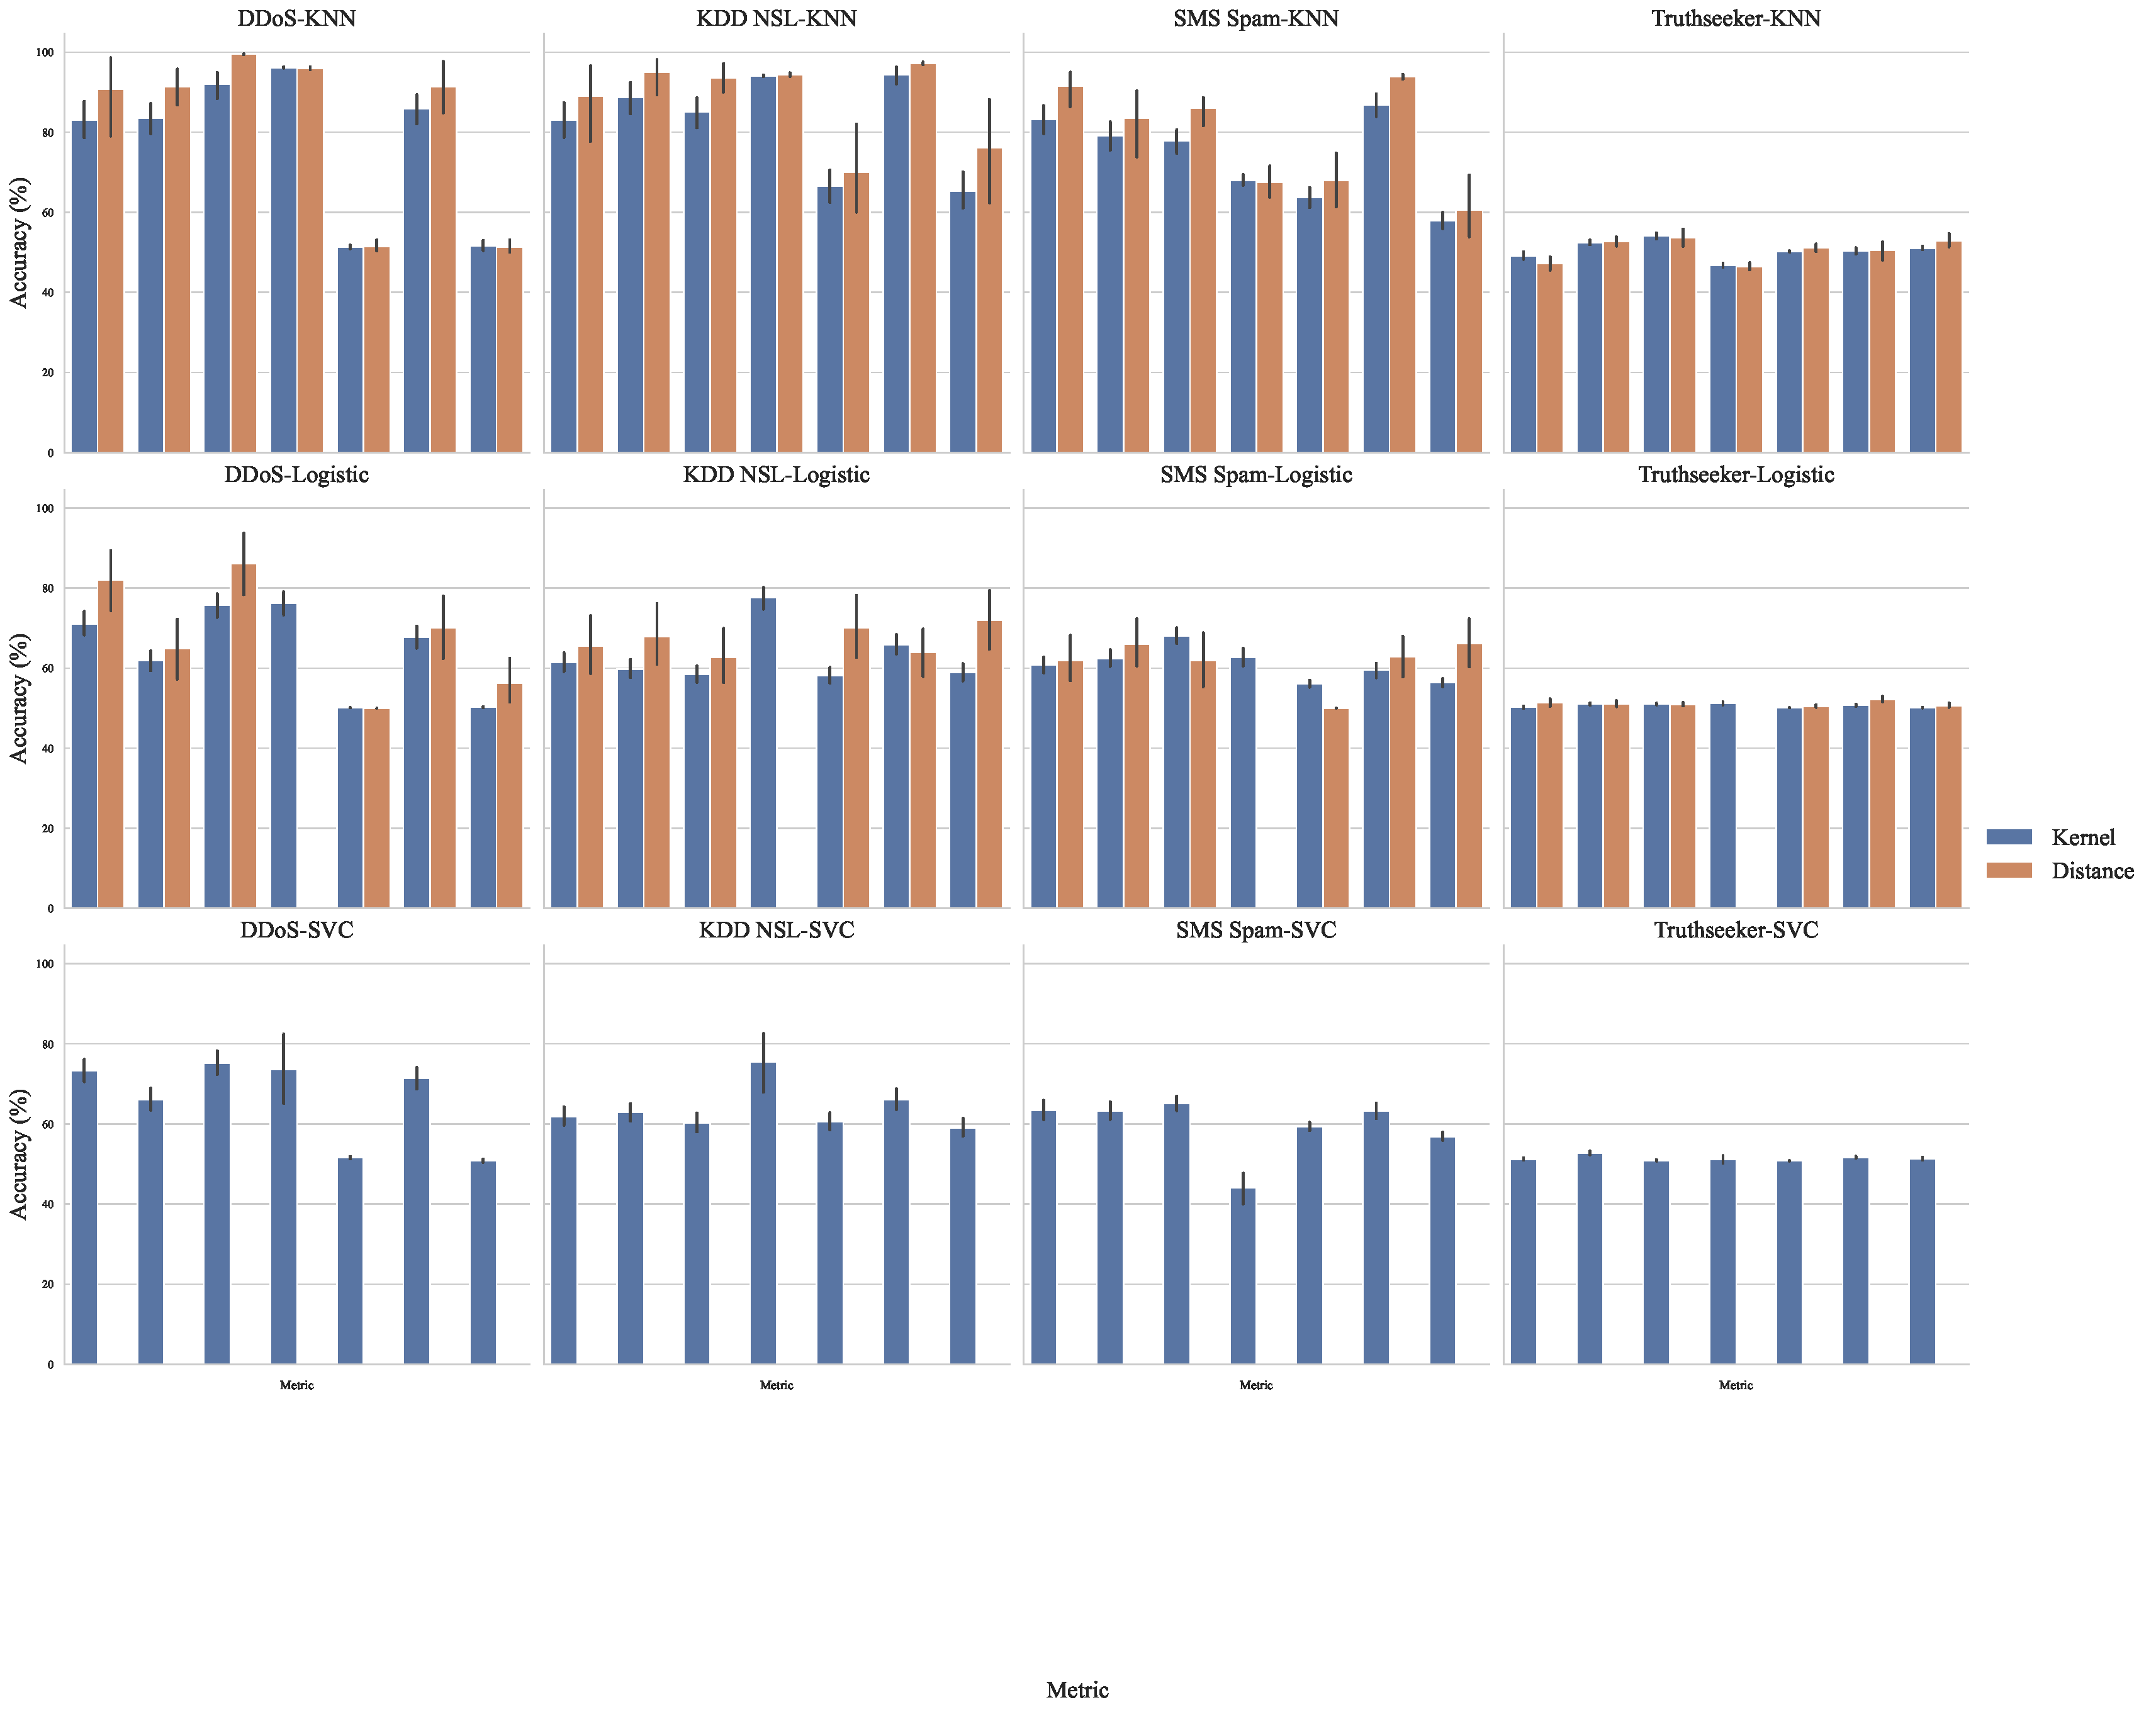
\includegraphics[width=0.99\textwidth]{images/accuracy_vs_kernel.pdf}
    \hfill
    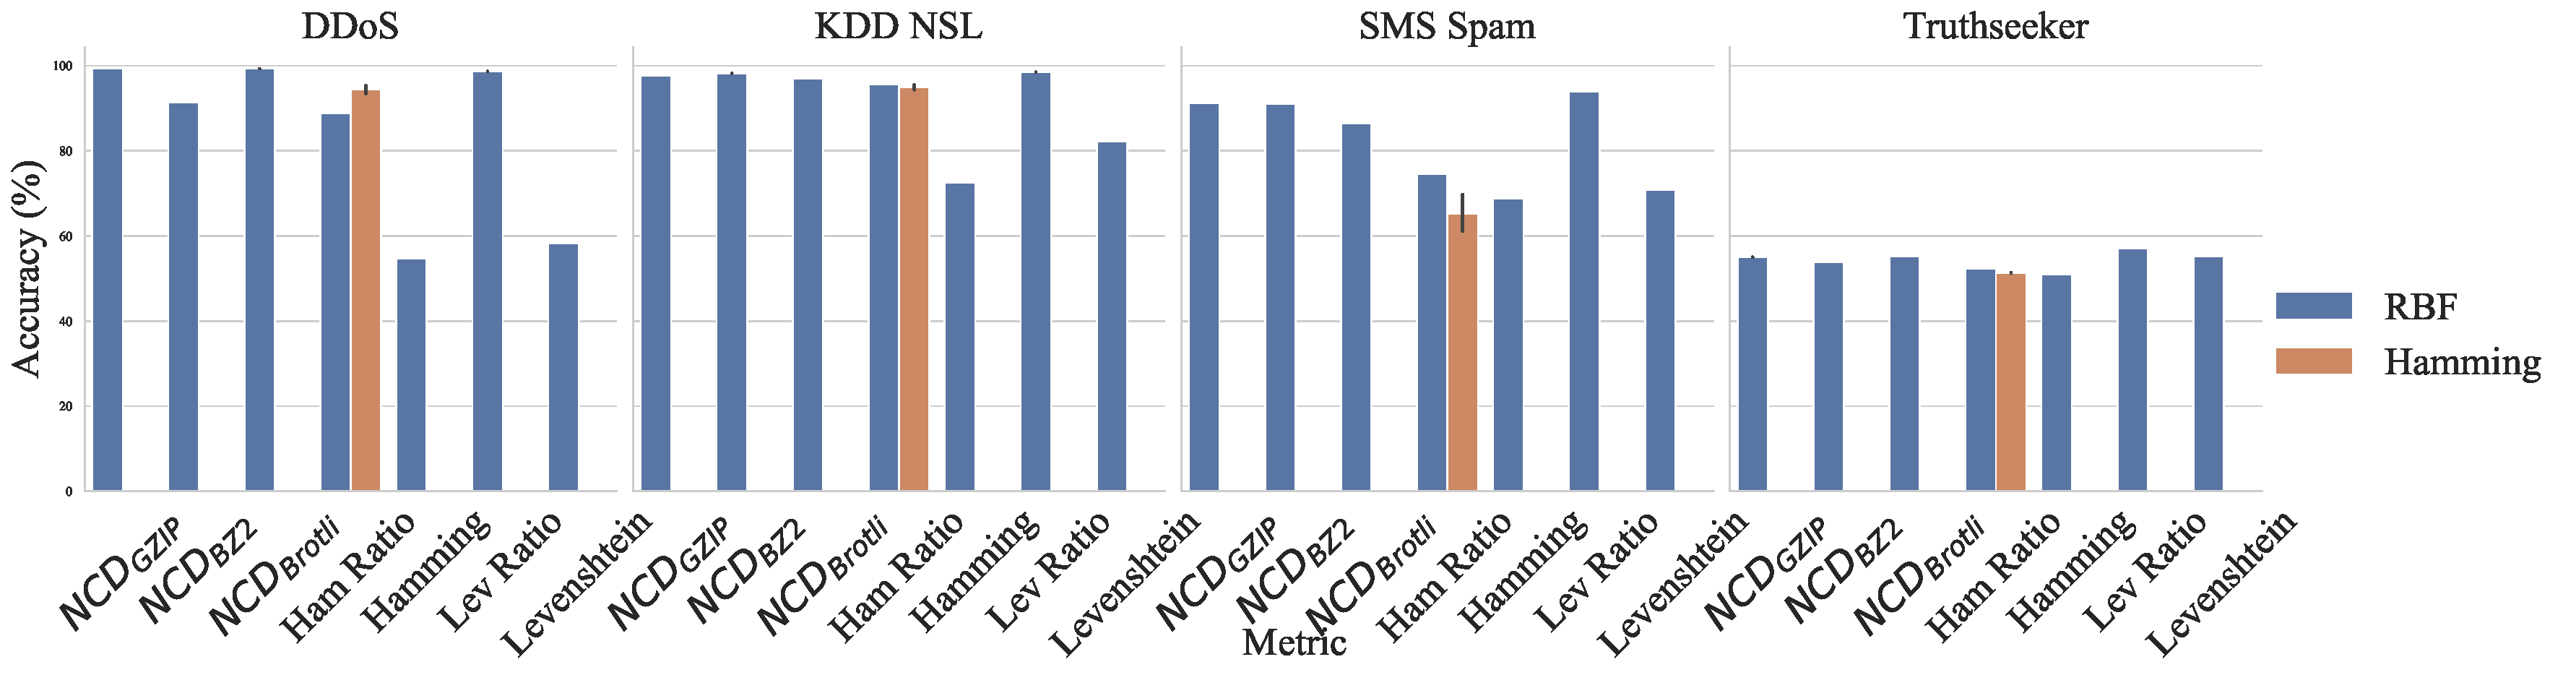
\includegraphics[width=0.99\textwidth]{images/accuracy_vs_rbf_or_hamming.pdf}
    \caption{
    The 5-fold accuracy across each dataset (columns), distance metric (first-axis), whether or not the distance or kernel matrix was used (top plot, colour), kernel (top plot, colour), and symmetrisation method (bottom plot, colour).
    Only KNN was used in the top plot as it is the only tested model that is meant to use distance matrices and the results depict the 5-fold accuracies for the best-fit model of each model-dataset-metric combination before (orange) and after kernelisation (blue).
    For both plots, the bars represent the mean accuracy and the error bars represent 95\% confidence intervals.
    }
    \label{fig:baseline}
\end{figure}


Figure~\ref{fig:baseline} depicts the mean accuracy of the best-fit model for each dataset-metric-model-kernel combination.
The error bars reflect the 95\% confidence interval of the mean accuracy, computed across five cross-validated folds.
The top of Figure~\ref{fig:baseline} compares accuracy of the proposed kernelised KNN to the distance-based KNN proposed by Jiang \textit{et al.}~\cite{jiang2022less} for a variety of string metrics (first axis).
The bottom of Figure~\ref{fig:baseline} compares the RBF kernel (Equation~\ref{eq:rbf_kernel}) to the Hamming kernel (Equation~\ref{eq:hamming_kernel}) for all three kernelised ML models.
It is clear that the kernel method is consistent with the distance method (top of Figure~\ref{fig:baseline}), apart from the un-normalised Levenshtein and Hamming distances, wherein the distance method is superior for the DDoS dataset.
Additionally, the RBF kernel has accuracy that is consistent with the Hamming kernel (bottom of Figure~\ref{fig:baseline}) and at least one version of NCD outperforms the Hamming ratio in every dataset.
Therefore, it is clear that the proposed kernelised classification model is as accurate at the distance-based KNN~\cite{jiang2022less} (top of Figure~\ref{fig:baseline}) and can also outperform the Hamming kernel (bottom of Figure~\ref{fig:baseline}).






\begin{figure}[!htb]
    \centering
    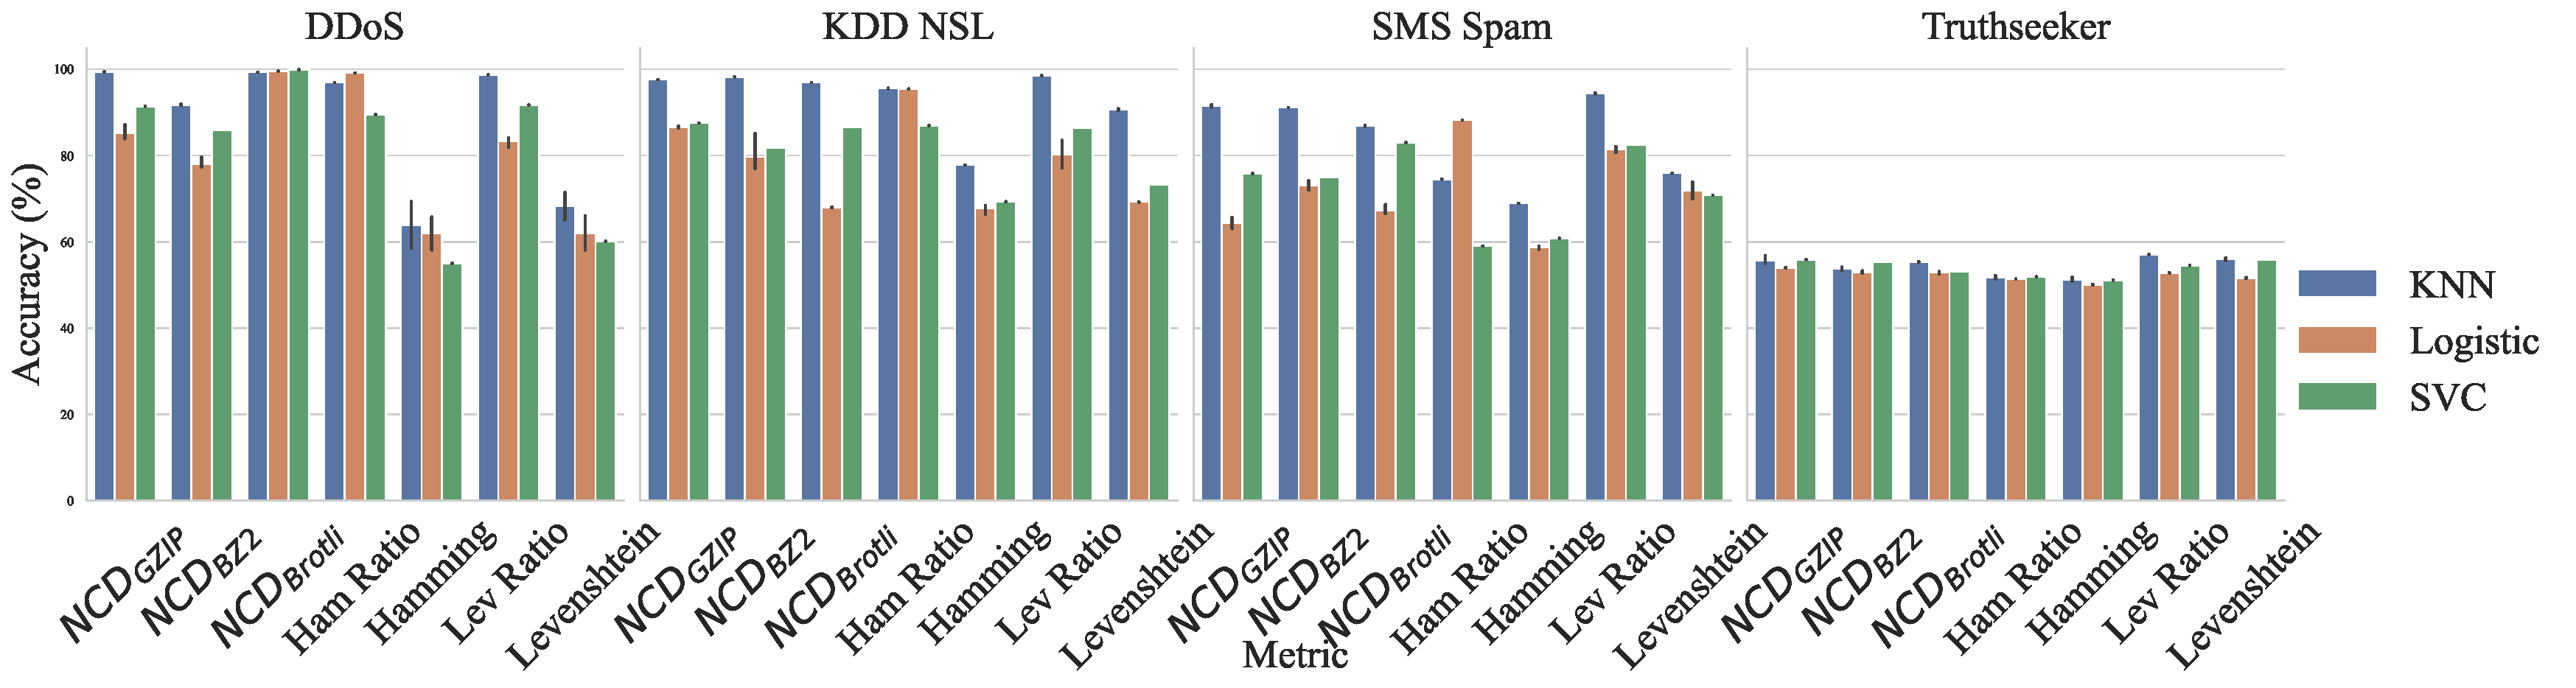
\includegraphics[width=0.99\textwidth]{images/accuracy_vs_metric.pdf}
    \hfill
    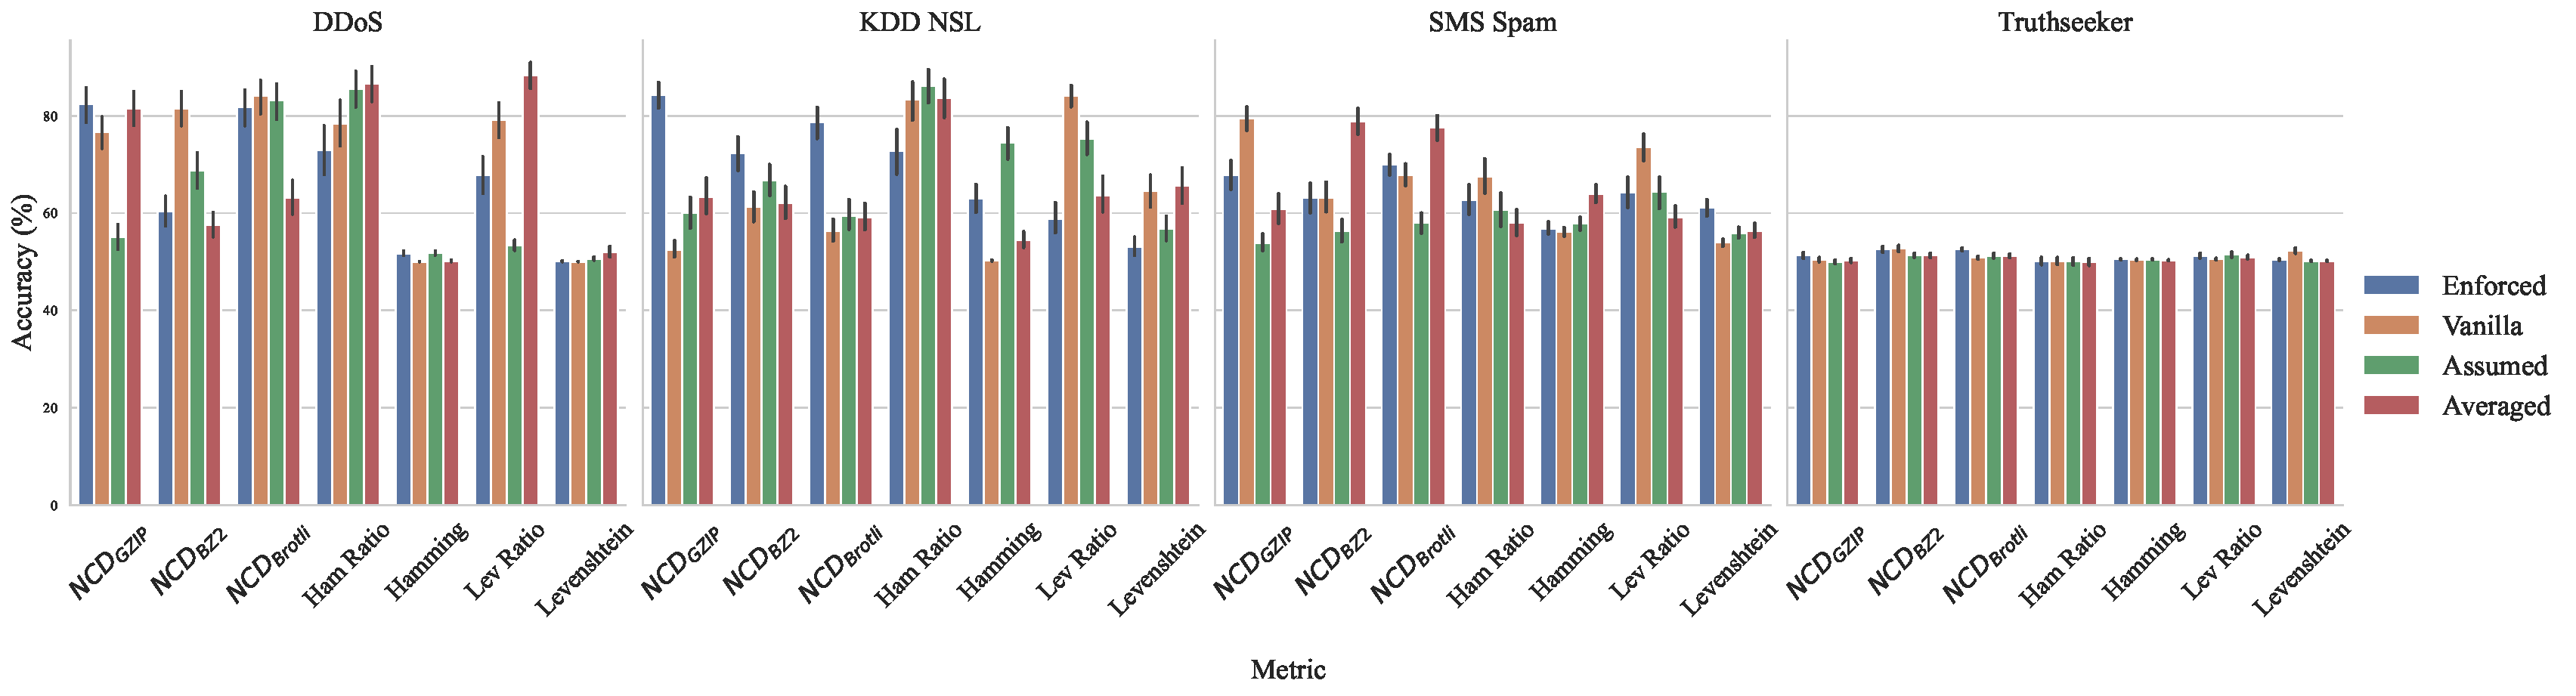
\includegraphics[width=0.99\textwidth]{images/accuracy_vs_symmetry.pdf}
    \caption{
    The accuracy across each dataset (columns), distance metric (first-axis),  model (top plot, colour), and symmetrisation method (bottom plot, colour).
    For both plots, the bars represent the mean accuracy and the error bars represent 95\% confidence intervals.
    }
    \label{fig:acc}
\end{figure}

Figure~\ref{fig:acc} shows the classifier performance across each dataset and string metric (including NCD, using various compressors) for both the kernel and distance matrices across all models (top row) and all symmetrisation methods (bottom row). 
The top sub-figure groups the results by model and the bottom figure groups the results by symmetrisation method.
From these results it is clear that KNN is the most consistently accurate (top of Figure~\ref{fig:acc}) and that symmetrisation method can be treated as a hyper-parameter, with optimal choice varying between dataset and model.

\begin{figure}[!bht]
    \centering
    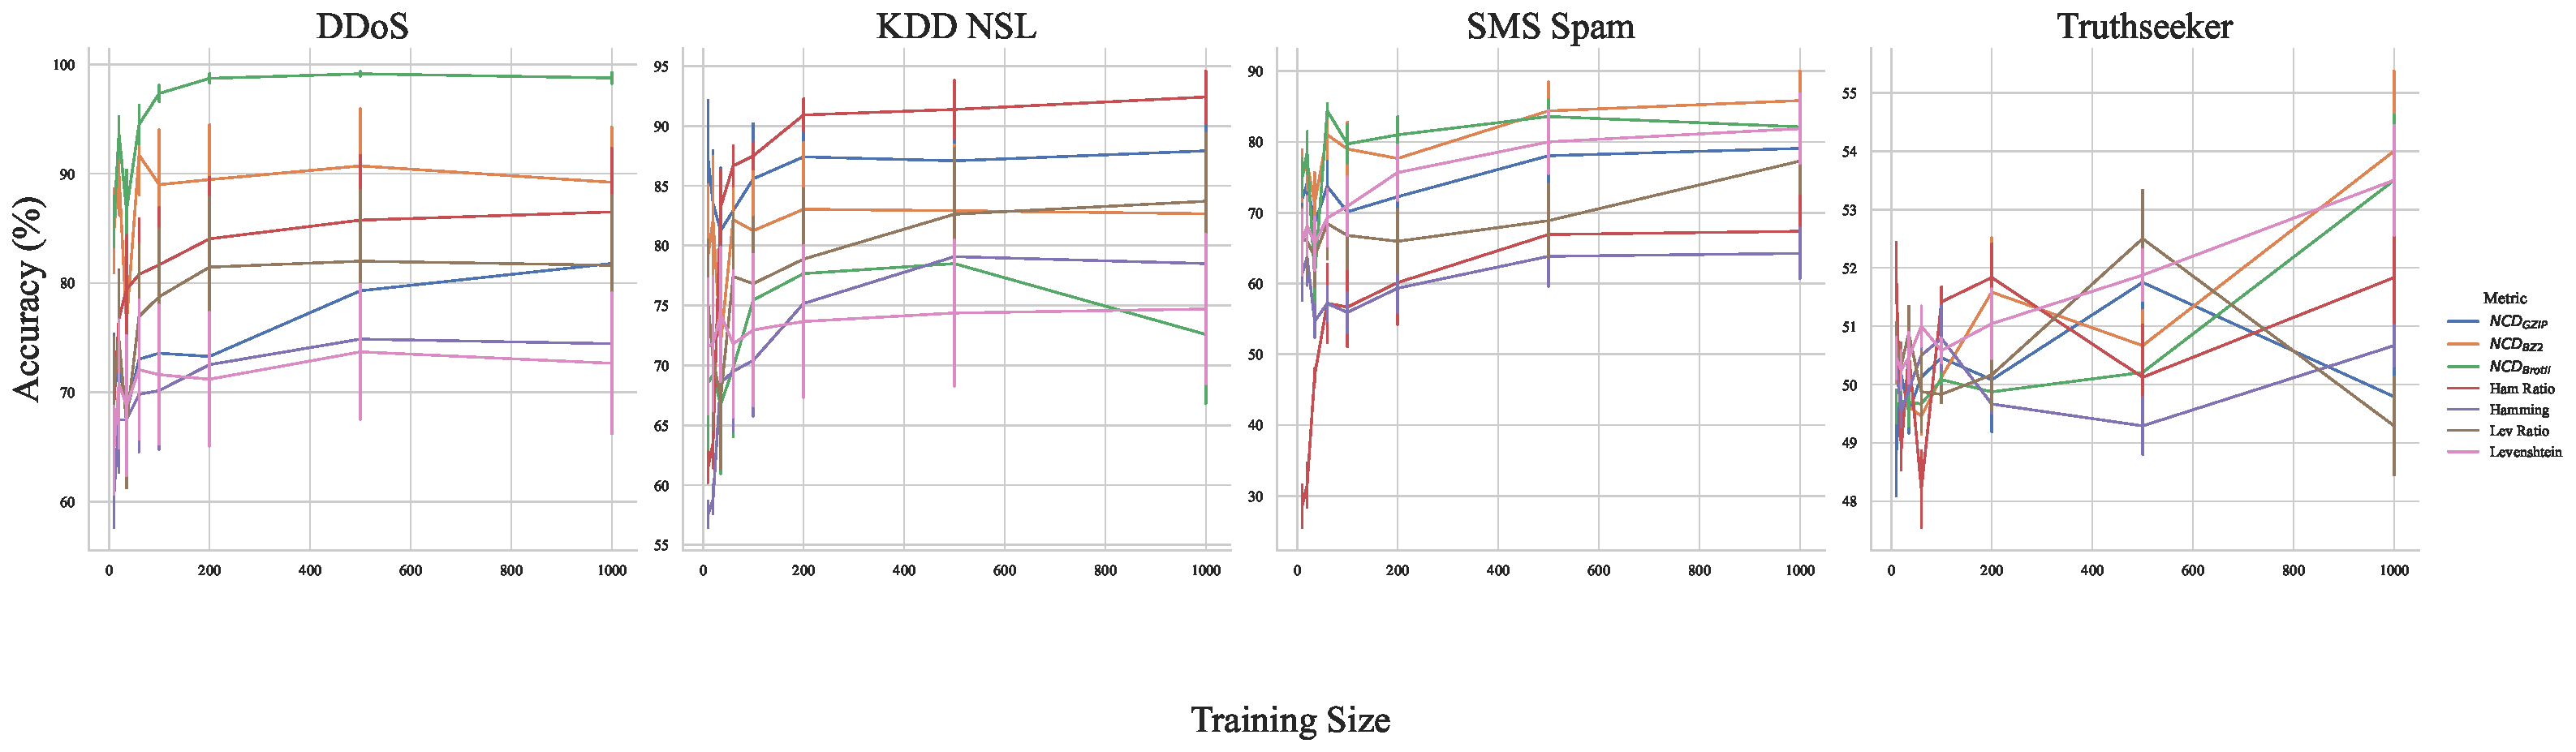
\includegraphics[width=\textwidth]{images/accuracy_vs_sample_size_vs_metric.pdf}
    \hfill
    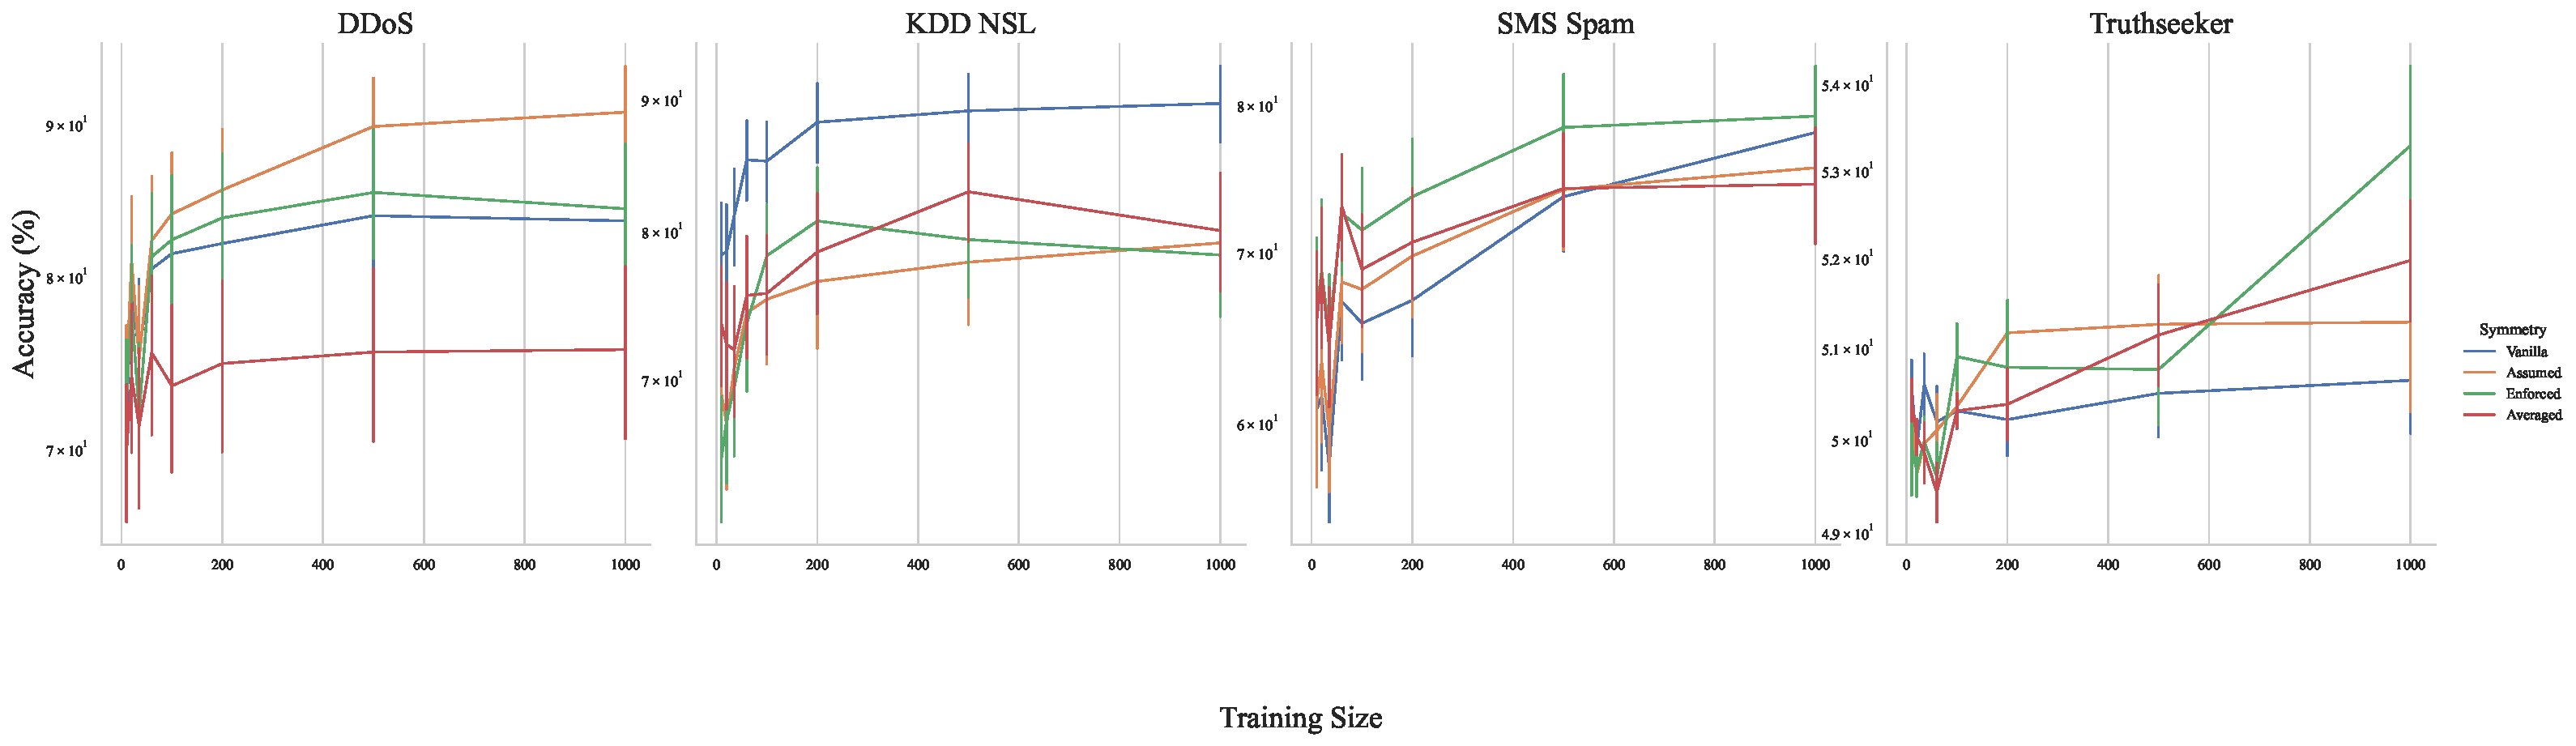
\includegraphics[width=\textwidth]{images/accuracy_vs_sample_size_vs_symmetric.pdf}
    \caption{
        Accuracy across varying training sample sizes, computed on 200 samples withheld during cross-validation using the best-fit model for each model–metric–symmetrisation configuration. \textit{Top:} Accuracy is grouped by evaluation metric (colour), showing how different metrics behave across datasets (columns) and training sizes, averaged over models and symmetrisation methods. \textit{Bottom:} Accuracy is grouped by symmetrisation method (colour), illustrating how different symmetrisation choices impact performance across datasets, averaged over models and metrics. Each line represents the mean accuracy, and error bars indicate the 95\% confidence interval of the mean.
    }
    \label{fig:sample_size}
\end{figure}

Figure~\ref{fig:sample_size} depicts the accuracy of the best-fit models as the number of training samples is varied (first-axis). 
The top of Figure~\ref{fig:sample_size} groups the results by metric and the bottom groups the results by symmetrisation method, using colour to differentiate the groups. 
For the DDoS dataset, it is clear from the top subplot of Figure~\ref{fig:sample_size} that NCD improves the accuracy when a small number of samples are used to train the model compared to other string metrics. 
However, results are more mixed for other datasets. 
Additionally, we can see that non-Vanilla symmetrisation methods tend to outperform the Vanilla variety on DDoS, SMS-Spam, and Truthseeker, although this is not significant.


\begin{figure}[htb!]
    \centering
    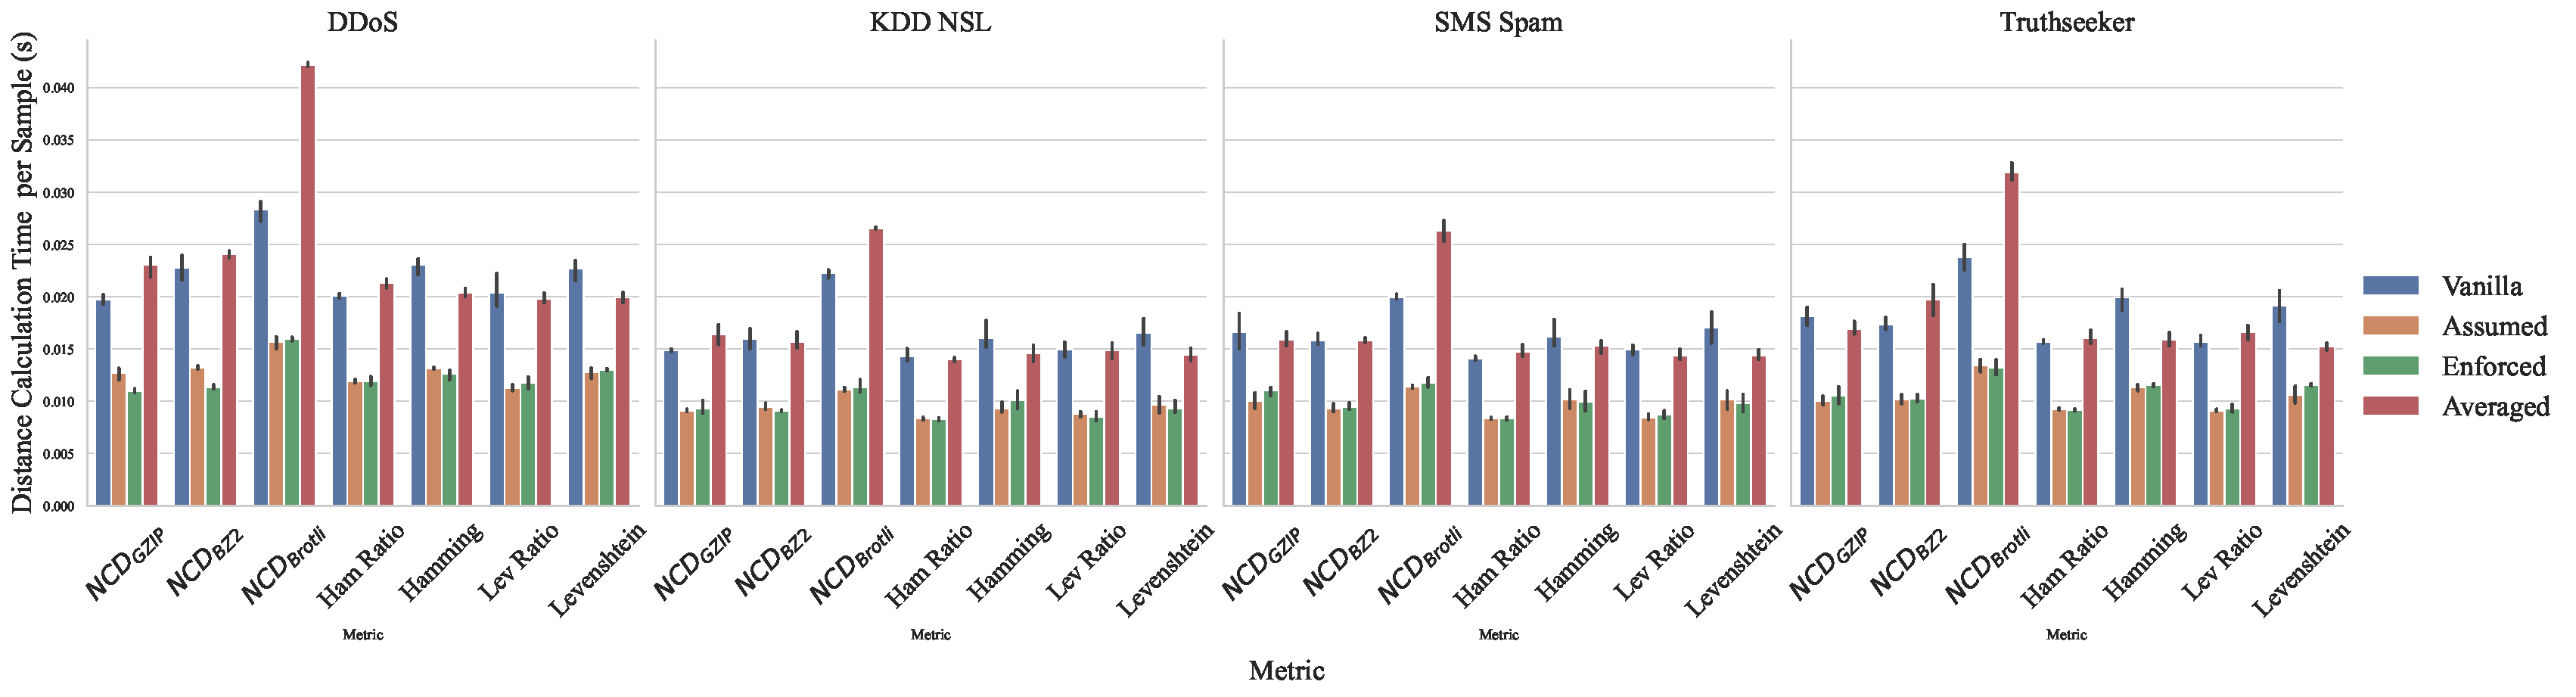
\includegraphics[width=0.99\textwidth]{images/distance_time_vs_symmetry.pdf}
    \hfill
    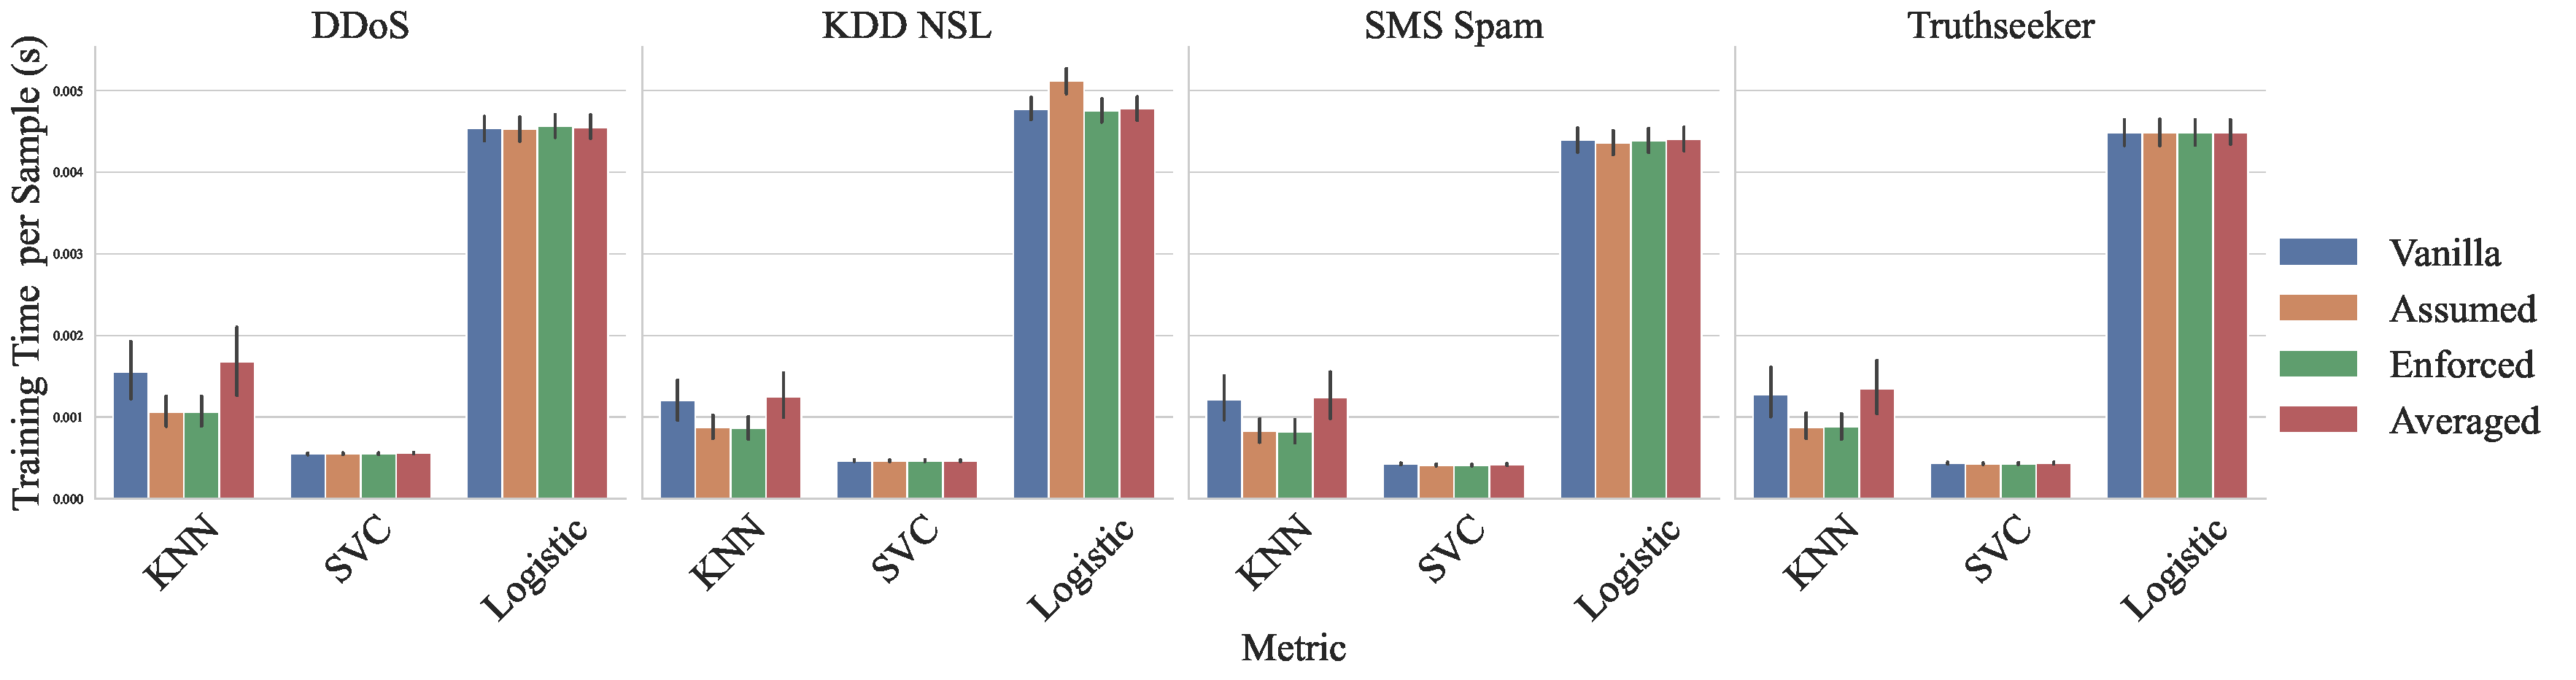
\includegraphics[width=0.99\textwidth]{images/train_time_vs_symmetry.pdf}
    \hfill
    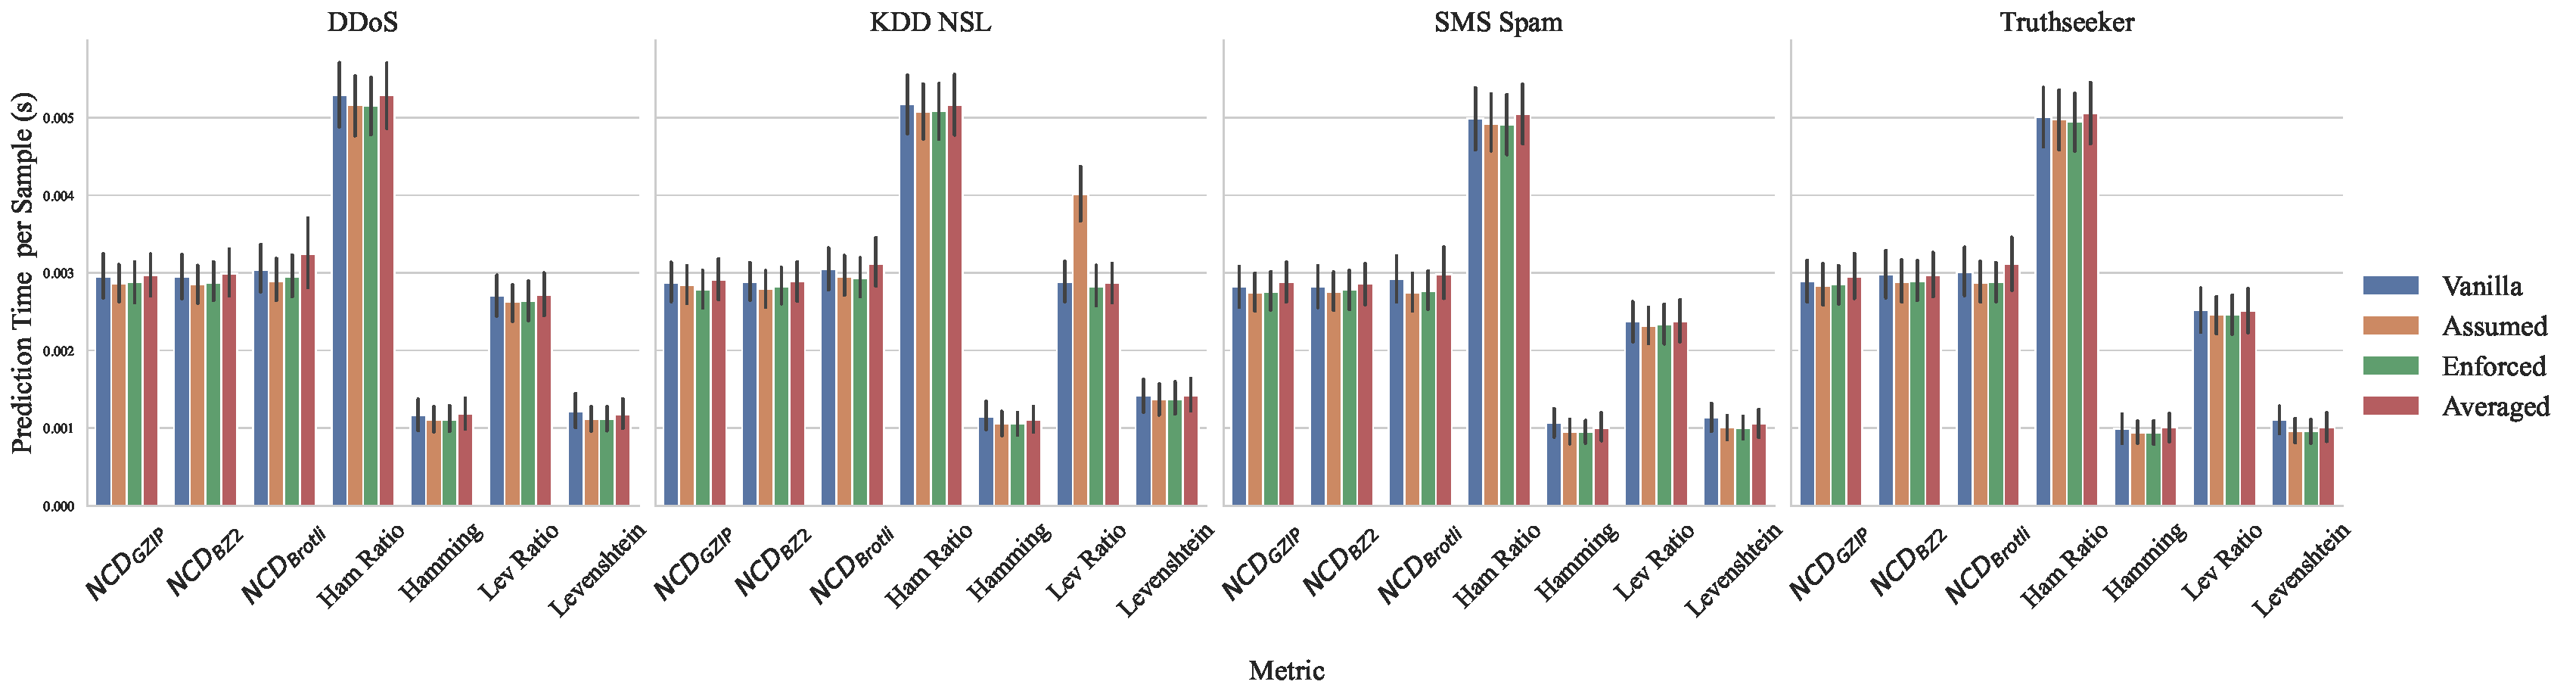
\includegraphics[width=0.99\textwidth]{images/pred_time_vs_symmetry.pdf}
    \caption{
        Performance times for various stages of the model evaluation process, computed across different metrics, datasets, and methods. \textit{Top:} Distance matrix calculation time per sample averaged over all dataset-method-metric combinations. \textit{Middle:} Training time per sample, measured after computing the distance matrix, averaged over all dataset-method-metric-model combinations. \textit{Bottom:} Prediction time per sample, also after distance matrix computation, showing the time required for predictions averaged over all dataset-method-metric-model combinations. For all three sub-plots, the colour reflects the symmetrisation method. The firs-axis shows the metric in the top and bottom plots, but the middle plot depicts the training time as it varies more by model than metric.
        The top of each bar reflects the mean of the measured time and the error bars are 95\% confidence intervals.
    }
    \label{fig:times}
\end{figure}



Figure~\ref{fig:times} shows the run-times associated with calculating the distance between two samples (top), training the model on a single sample (middle), or inferring the classification of a new sample (bottom).
The importance of the symmetrisation methods is to reduce the run-time.
It is clear from Figure~\ref{fig:times} that choice of symmetrisation method has a substantial effect on run-time, with the ``Assumed'' and ``Enforced'' symmetrisation methods taking roughly half as long per sample as the ``Vanilla'' version and the ``Averaged'' version taking slightly longer.
During training (assuming the distance or kernel-matrix is pre-computed), the variance between models is far large than the variance induced by the symmetrisation methods (see middle row of Figure~\ref{fig:times}).
During prediction, the differences between symmetrisation methods are much less pronounced, owing to the smaller number of samples---instead, the variance in prediction times is predominated by the run-time of the distance function as the variance within a given metric is much smaller than the variance between them (see the bottom row of Figure~\ref{fig:times}).

\begin{figure}[ht!]
    \centering
    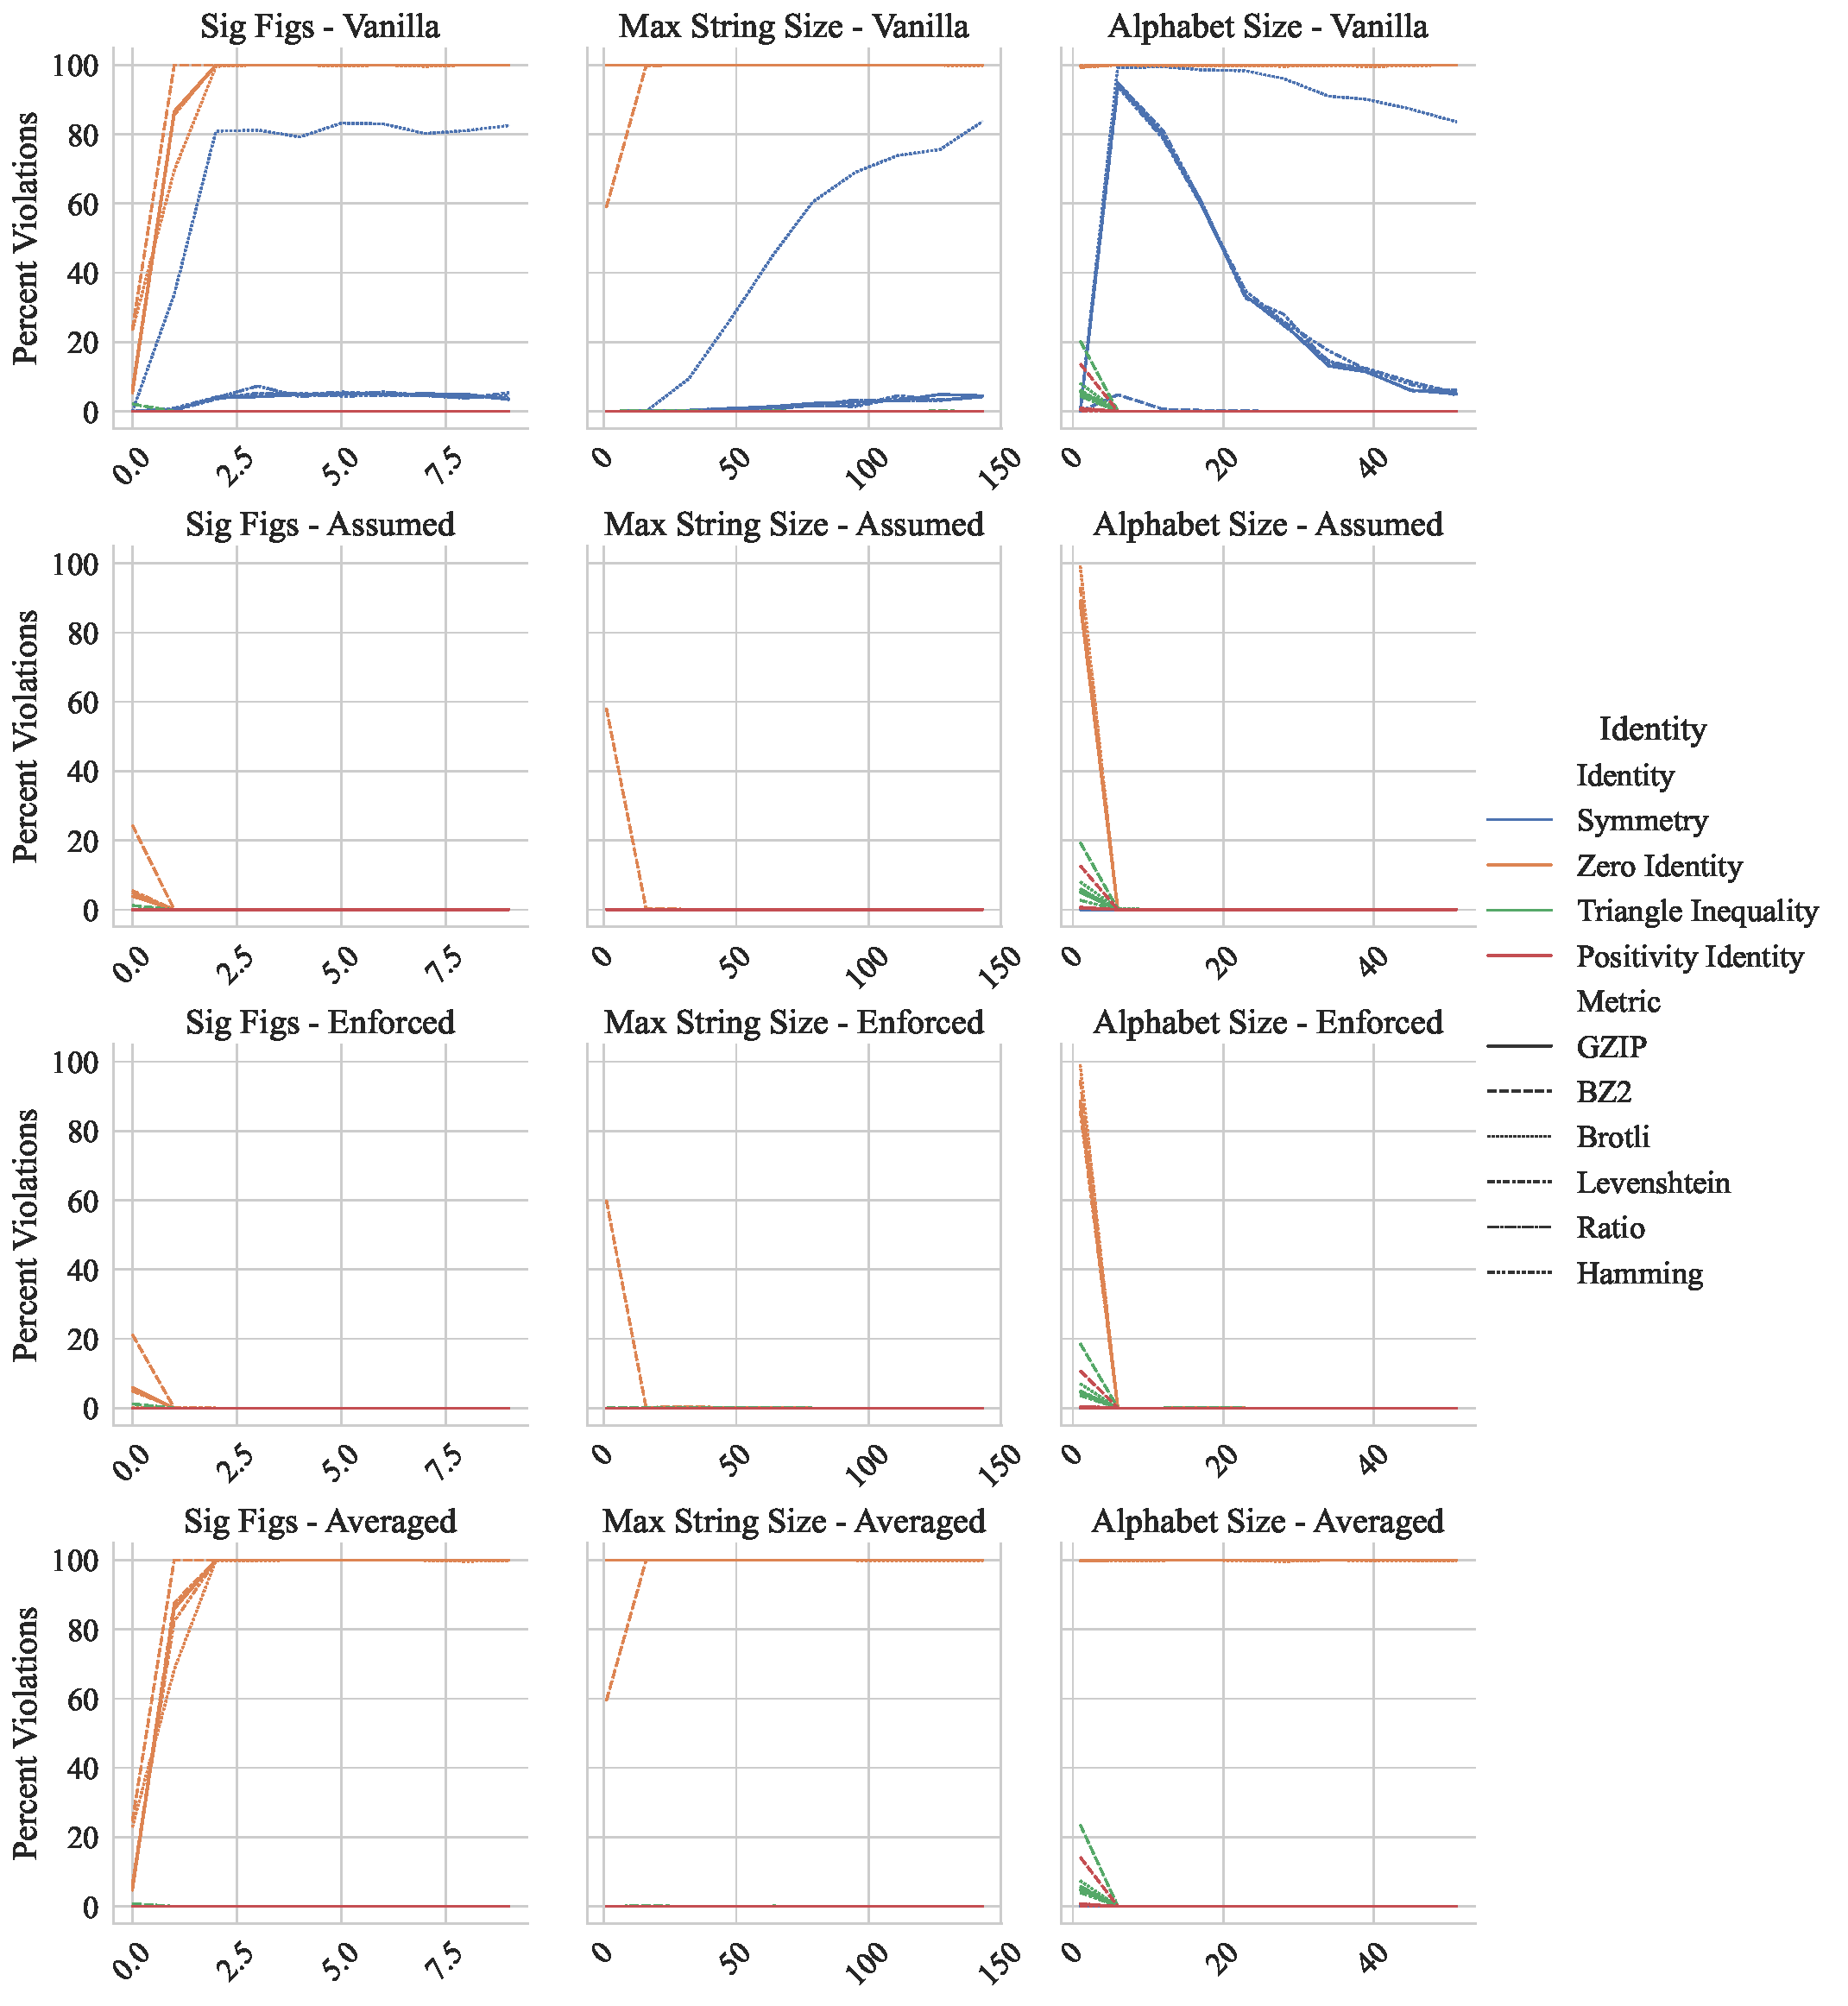
\includegraphics[width=\textwidth]{images/synthetic_check.pdf}
    \caption{
   Percentage of violations of Axioms~\ref{eq:axiom_zero}--\ref{eq:axiom_triangle} among 100,000 random strings (from the standard English alphabet), using four symmetrisation methods: vanilla, assumed symmetry, enforced symmetry, and averaging. The top plots vary max string size; bottom plots vary alphabet size. Default settings: max string size is 144, alphabet size is 26. Colours indicate axioms; solid lines indicate NCD (Equation~\ref{eq:ncd}) and dashed lines are for other string metrics (Section~\ref{other_string_metrics}).
    }
    \label{fig:synthetic_check}
\end{figure}

\begin{figure}[p!]
    \centering
    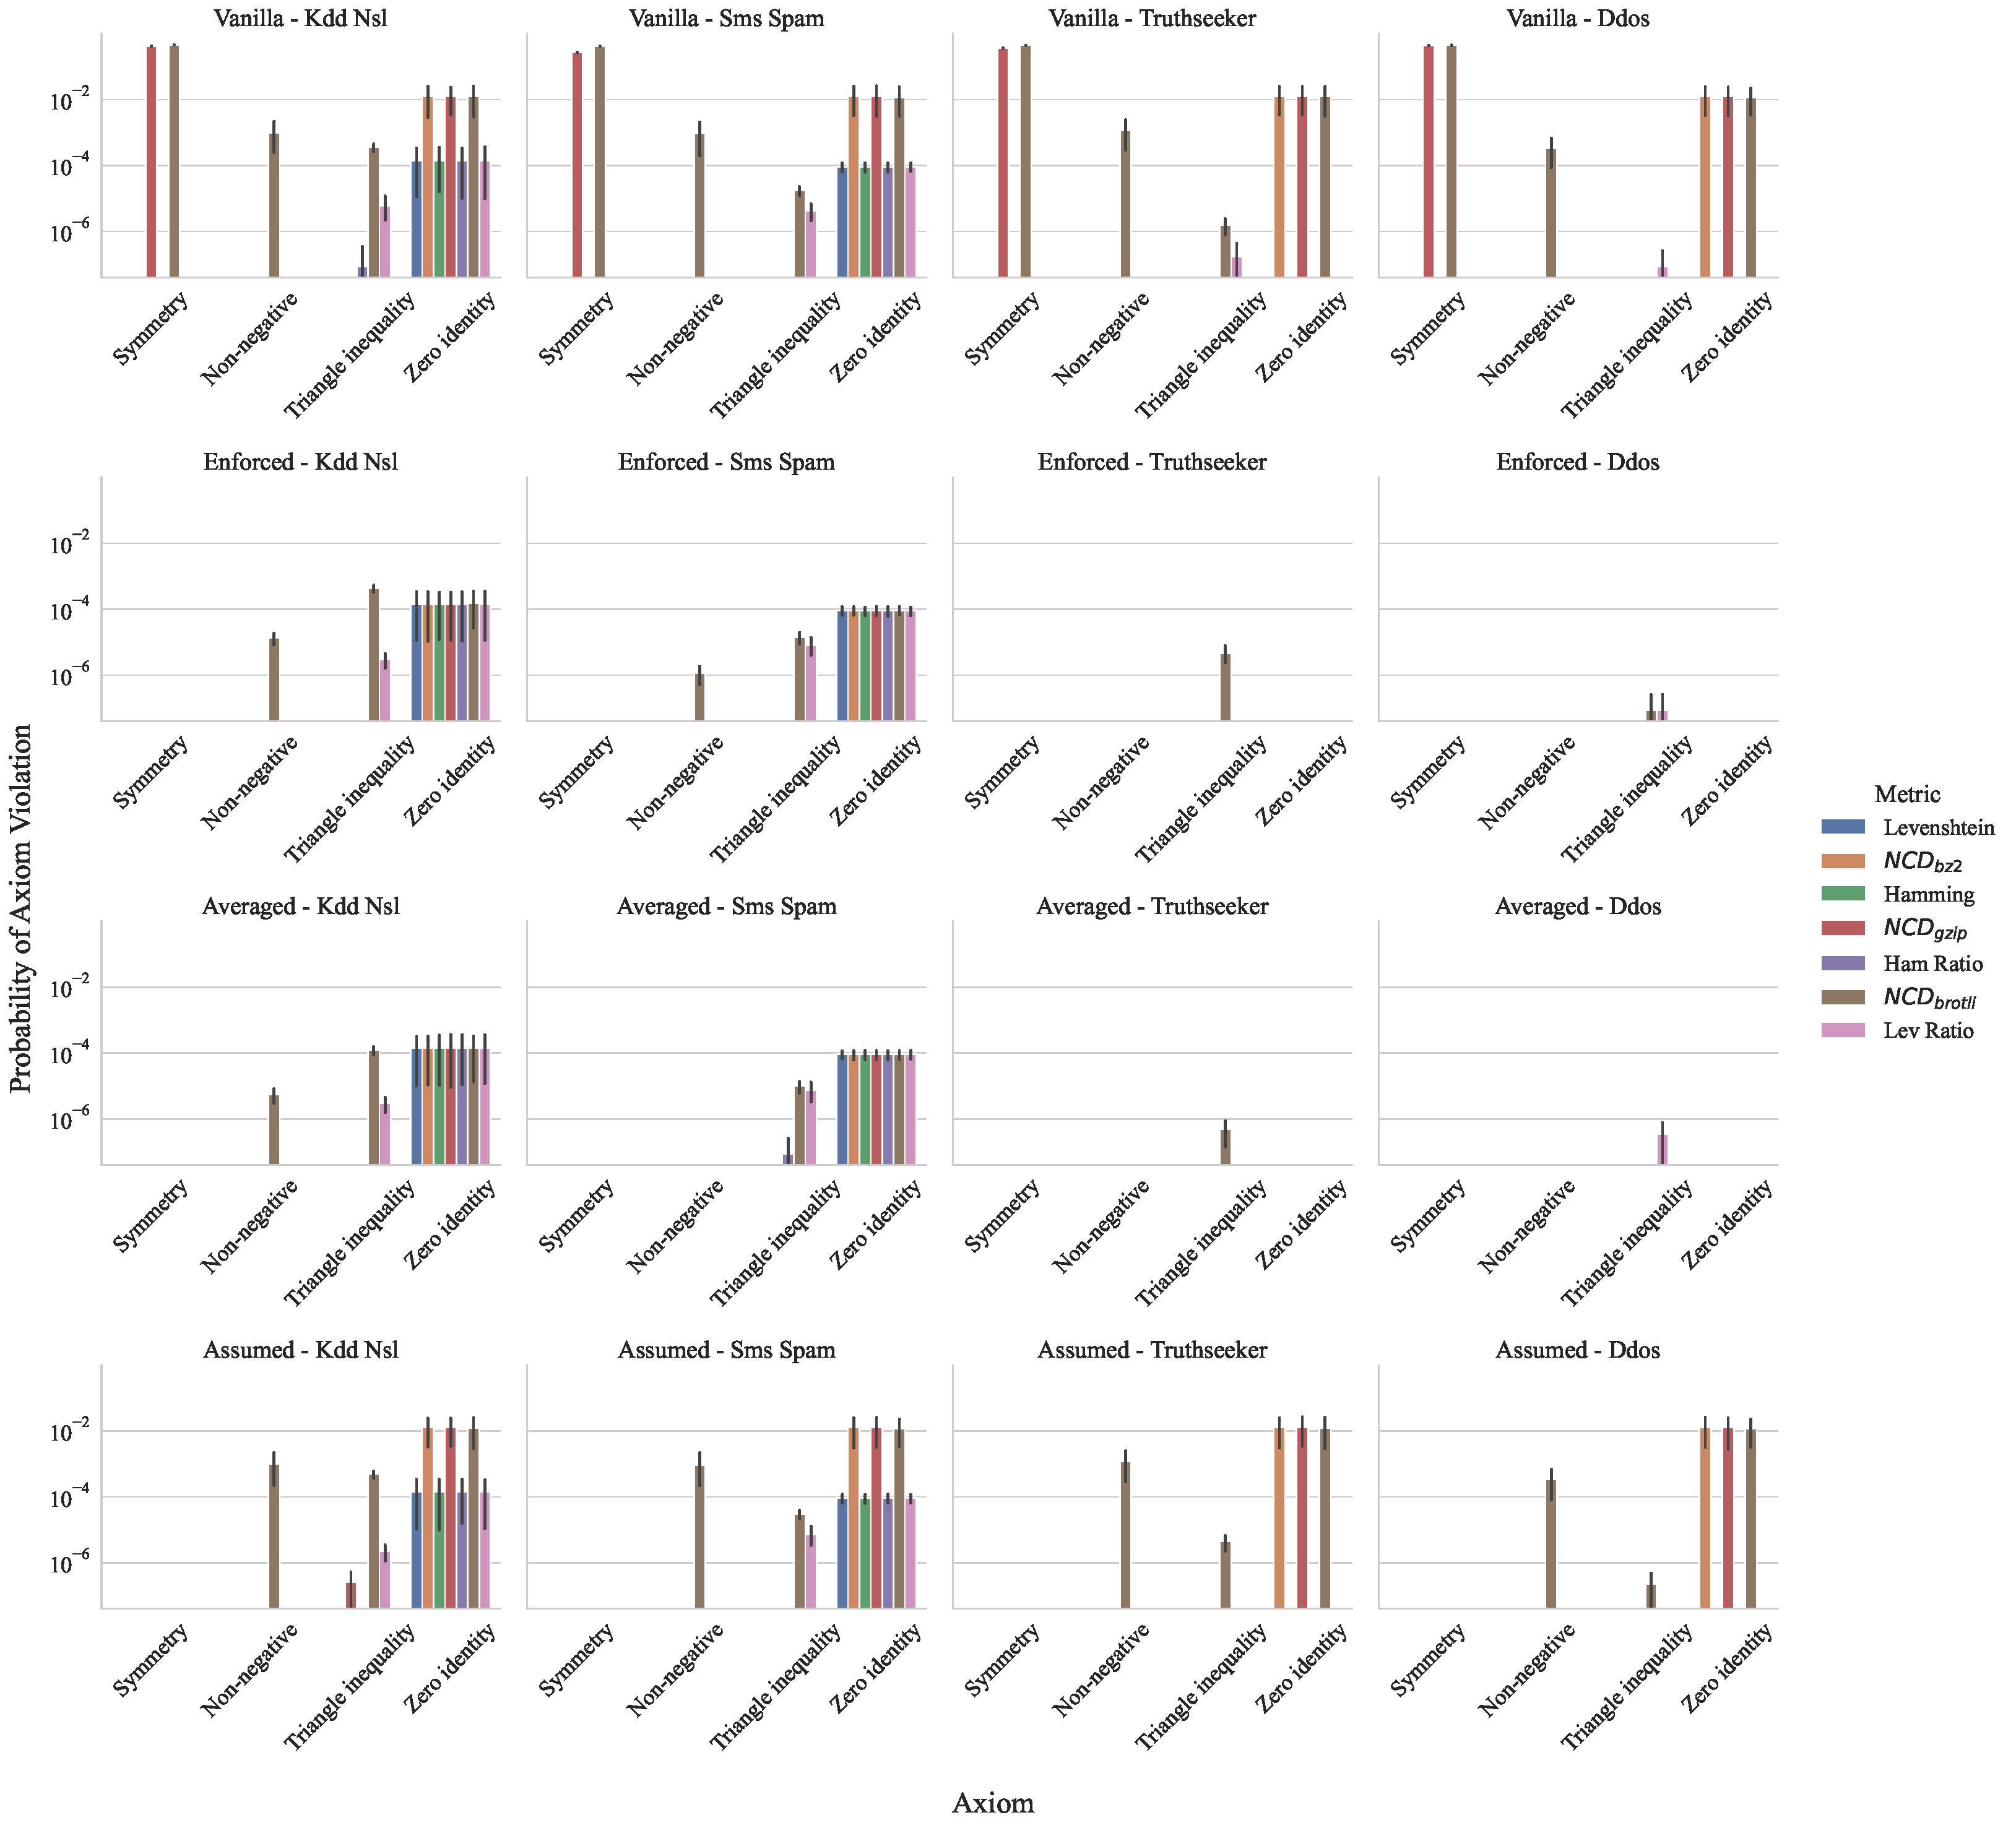
\includegraphics[width=0.99\textwidth]{images/real_world_check.pdf}
    \caption{
    Percentage of examples found that violate the assumptions outlined in Equations~\ref{eq:axiom_zero}--\ref{eq:axiom_triangle} using the vanilla (top row), assumed symmetry (second row), enforced (third row), and averaged (bottom row) methods on the training matrices for each of the outlined datasets. Each column is dedicated to a dataset and each model is given a column. The first axis displays which of the axioms is violated and the colour indicates which symmetrisation method was used. Since evaluating all possible distance 3-tuples would be computationally infeasible for even hundreds of samples, three samples were sampled  100 thousand times such that no 3-tuple was repeated.
    }
    \label{fig:real_world_check}
\end{figure}

Figures~\ref{fig:synthetic_check}--\ref{fig:real_world_check} display how the symmetrisation methods influence to what degree a given metric adheres to the axioms outlined in Equations~\ref{eq:axiom_zero}--\ref{eq:axiom_triangle} and show that they enforce adherence to the symmetric and zero-axiom as expected.
It is clear from these figures that the averaging, enforcing, or assuming symmetry works quite well, thus fulfilling Equation~\ref{eq:axiom_symmetry}.
Likewise, Equation~\ref{eq:axiom_zero} acts as expected (compare ``Vanilla'' and ``Averaged'' with the other two methods). 
This is true on randomly constructed strings (Figure~\ref{fig:synthetic_check}) as well as strings collected from the aforementioned datasets (Figure~\ref{fig:real_world_check}). 
It is clear that this does not correspond to a decrease in accuracy (see Figure~\ref{fig:acc}) and that these modifications can significantly improve run-time (see Figure~\ref{fig:times} in Figures~\ref{fig:synthetic_check}--\ref{fig:real_world_check}).


\section{Limitations}
\label{limitations}
While the methods presented in this work demonstrate strong performance across various tasks and datasets, several limitations should be acknowledged.

To further improve run-time performance, compression algorithms optimised for graphics processing units (GPUs) have been developed~\cite{gpu_compression}.
These are likely to outperform the CPU-based implementations used in this paper when applied to large-scale datasets.
Incorporating such GPU-accelerated compressors could significantly reduce processing time and improve scalability.

The model tuning parameters used in this study were limited in scope.
While the selected configurations were sufficient to demonstrate key insights, a broader hyperparameter search may reveal additional trade-offs or improvements in accuracy and efficiency.

This work focused on a specific set of compression algorithms.
Although other compressors exist--including those optimised for specific data types~\cite{gpu_compression,mp3,hevc}—-they were considered out of scope for this study.
Future work could explore the impact of alternative compressors on both accuracy and run-time.
Likewise, the data preprocessing step used for heterogeneous tabular data was intentionally kept simple---each row was cast to a Python list then cast again as a string. 
While effective for our purposes (see Figure~\ref{fig:baseline}), this approach is crude and may obscure structural or semantic relationships within the data by including extraneous characters like commas and brackets (used to delineate and denote a list in Python, respectively).
As always, the best implementation will be determined by the data and its schema.
More sophisticated encoding methods—such as schema-aware parsing or embedding techniques—could improve performance, particularly on more complex or high-dimensional datasets.




\section{Conclusion}
\label{conclusion}

Overall, we see that NCD is at least as accurate as other string metrics (top of Figure~\ref{fig:acc}), despite not being a true metric (Lemma~\ref{pseudometric}).
Furthermore, we see that the proposed symmetrisation methods are quite effective---sometimes even outperforming the ``Vanilla'' method (bottom of Figure~\ref{fig:acc}).
Kernelised NCD is effective even when only a small number of samples are used to train the model, making it ideal for lightweight, client-side deployments (top of Figure~\ref{fig:sample_size}) and our extensions (Section~\ref{improvements}) do not significantly change this result (bottom of Figure~\ref{fig:sample_size}).
NCD can reach more than 95\% accuracy on even tens of samples (Figure~\ref{fig:sample_size}).
It is clear from Figure~\ref{fig:times} that the ``Assumed'' and ``Enforced'' symmetrisation methods proposed in this work are superior to those found in the literature by decreasing the run-time without penalising accuracy (bottom of Figure~\ref{fig:acc}).
In some cases, the ``Averaged'' symmetrisation method offers superior accuracy over the other methods (Figure~\ref{fig:acc}, bottom) while inducing a marginal cost of only a few milliseconds (Figure~\ref{fig:times}, top).
In other cases, ``Enforced'' and ``Assumed'' offer both superior accuracies (Figure~\ref{fig:acc}, bottom) and run-times (Figure~\ref{fig:times}, top and bottom).

The proposed model is a real-time, client-side classification method that can be trained on a very small number of samples---potentially collected from only a single user.
This reduces the attack surface to only adversaries that have access to data that users generally consider private (\textit{e.g.}, the contents of a message).
That is, the attack surface is reduced and can be unique to each user, session, or device by using data from each user in isolation and training a model on that user's device. Client-side models would only need to share a single bit (the classification label in a binary classification context) with the platform operator---allowing those operators to serve user-specific contents without exfiltrating private data from their entire user base.
However, not training a model on large amounts of collected user data means that such hypothetical client-side methods are at risk of not performing at the level of state-of-the-art large-scale methods.
% By training a model for each user, session, and/or device, model database poisoning attacks~\cite{biggio_poisoning_2013} are categorically avoided.
% Furthermore, the proposed model reduces the attack surface of attacks like model inference attacks, database exfiltration attacks, and evasion attacks since a malicious user would need to target the personalised classifier of each user session, and/or device~\cite{biggio_evasion_2013,deepfool,chakraborty_adversarial_2018,extraction_attack}.
% While it is known that some attacks are quite transferable~\cite{wang2021enhancing}, the proposed model reduces the common attack surface to \textit{only} samples that are universal for all users.
The end result is a model with a substantially reduced attack surface that is nevertheless accurate, but also simple, generally applicable, and very fast.



\bibliographystyle{elsarticle-num}
\bibliography{bibliography}

\end{document}
